\documentclass[12pt]{article}
\usepackage[letterpaper, left=15mm, right=15mm, top=21mm, bottom=19mm, headheight=15pt, headsep=5mm, footskip=9mm]{geometry}
\usepackage[T1]{fontenc}
\usepackage{tgheros}
\renewcommand{\familydefault}{\sfdefault}
\usepackage{tikz}
\usepackage{fancyhdr}
\pagestyle{fancy}
\fancyhf{}
\lhead{Week 53 / Connecting networks / Grades 4--5}
\lfoot{\small Bellingham Math Circle / Week 53 / W53-RV-U-v1}
\rfoot{\small \thepage}
\renewcommand{\headrulewidth}{0.4pt}
\setlength{\parindent}{0pt}
\setlength{\parskip}{0pt}
\linespread{1.06}
\newcommand{\prob}[1]{\textbf{Problem #1:}}
\newcommand{\ans}[1]{\rule[-0.6ex]{#1}{0.5pt}}
\begin{document}

Buy a link by laying a marker along it and putting its price in counters in the tray. A network is a set of bought links that lets the pawn walk on markers between every two circled places. A network may pass through places in squares or leave them out. A route is a way to walk from one place to another along links, written by its letters, such as ABD.

\vspace{3mm}
\prob{1} For each pair of places below, find a route whose most expensive link is as cheap as possible.

\par\begin{center}
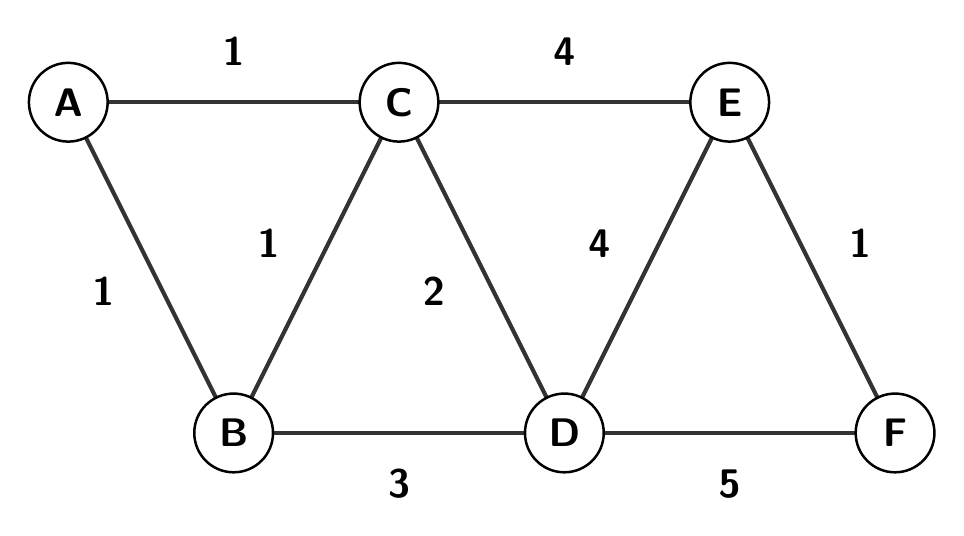
\begin{tikzpicture}[x=1mm,y=1mm]
\draw[line width=1.5pt, black!80] (5.00,51.46) -- (26.00,9.46);
\draw[line width=1.5pt, black!80] (5.00,51.46) -- (47.00,51.46);
\draw[line width=1.5pt, black!80] (26.00,9.46) -- (47.00,51.46);
\draw[line width=1.5pt, black!80] (47.00,51.46) -- (68.00,9.46);
\draw[line width=1.5pt, black!80] (26.00,9.46) -- (68.00,9.46);
\draw[line width=1.5pt, black!80] (47.00,51.46) -- (89.00,51.46);
\draw[line width=1.5pt, black!80] (68.00,9.46) -- (89.00,51.46);
\draw[line width=1.5pt, black!80] (89.00,51.46) -- (110.00,9.46);
\draw[line width=1.5pt, black!80] (68.00,9.46) -- (110.00,9.46);
\node[fill=white, inner sep=0, minimum width=4.40mm, minimum height=6.00mm, font=\Large\bfseries] at (9.44,27.44) {1};
\node[fill=white, inner sep=0, minimum width=4.40mm, minimum height=6.00mm, font=\Large\bfseries] at (26.00,57.93) {1};
\node[fill=white, inner sep=0, minimum width=4.40mm, minimum height=6.00mm, font=\Large\bfseries] at (30.44,33.49) {1};
\node[fill=white, inner sep=0, minimum width=4.40mm, minimum height=6.00mm, font=\Large\bfseries] at (51.44,27.44) {2};
\node[fill=white, inner sep=0, minimum width=4.40mm, minimum height=6.00mm, font=\Large\bfseries] at (47.00,3.00) {3};
\node[fill=white, inner sep=0, minimum width=4.40mm, minimum height=6.00mm, font=\Large\bfseries] at (68.00,57.93) {4};
\node[fill=white, inner sep=0, minimum width=4.40mm, minimum height=6.00mm, font=\Large\bfseries] at (72.44,33.49) {4};
\node[fill=white, inner sep=0, minimum width=4.40mm, minimum height=6.00mm, font=\Large\bfseries] at (105.56,33.49) {1};
\node[fill=white, inner sep=0, minimum width=4.40mm, minimum height=6.00mm, font=\Large\bfseries] at (89.00,3.00) {5};
\node[circle, draw, line width=0.9pt, fill=white, minimum size=10.00mm, inner sep=0, font=\Large\bfseries] at (5.00,51.46) {A};
\node[circle, draw, line width=0.9pt, fill=white, minimum size=10.00mm, inner sep=0, font=\Large\bfseries] at (47.00,51.46) {C};
\node[circle, draw, line width=0.9pt, fill=white, minimum size=10.00mm, inner sep=0, font=\Large\bfseries] at (89.00,51.46) {E};
\node[circle, draw, line width=0.9pt, fill=white, minimum size=10.00mm, inner sep=0, font=\Large\bfseries] at (26.00,9.46) {B};
\node[circle, draw, line width=0.9pt, fill=white, minimum size=10.00mm, inner sep=0, font=\Large\bfseries] at (68.00,9.46) {D};
\node[circle, draw, line width=0.9pt, fill=white, minimum size=10.00mm, inner sep=0, font=\Large\bfseries] at (110.00,9.46) {F};
\end{tikzpicture}
\end{center}\par

\vspace{4mm}
\begin{center}
\begin{tabular}{@{}l@{\hspace{3mm}}l@{\hspace{8mm}}l@{}}
A to D: & route \ans{40mm} & most expensive link \ans{14mm}\\[9mm]
B to D: & route \ans{40mm} & most expensive link \ans{14mm}\\[9mm]
D to F: & route \ans{40mm} & most expensive link \ans{14mm}\\[9mm]
A to F: & route \ans{40mm} & most expensive link \ans{14mm}
\end{tabular}
\end{center}
\newpage

\prob{2} Find every cheapest network on this map.

\par\begin{center}
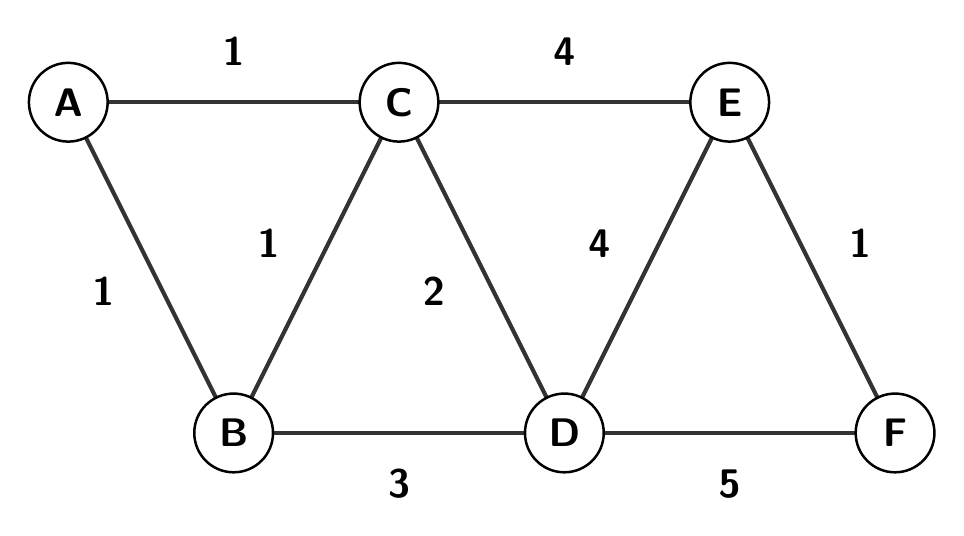
\begin{tikzpicture}[x=1mm,y=1mm]
\draw[line width=1.5pt, black!80] (5.00,51.46) -- (26.00,9.46);
\draw[line width=1.5pt, black!80] (5.00,51.46) -- (47.00,51.46);
\draw[line width=1.5pt, black!80] (26.00,9.46) -- (47.00,51.46);
\draw[line width=1.5pt, black!80] (47.00,51.46) -- (68.00,9.46);
\draw[line width=1.5pt, black!80] (26.00,9.46) -- (68.00,9.46);
\draw[line width=1.5pt, black!80] (47.00,51.46) -- (89.00,51.46);
\draw[line width=1.5pt, black!80] (68.00,9.46) -- (89.00,51.46);
\draw[line width=1.5pt, black!80] (89.00,51.46) -- (110.00,9.46);
\draw[line width=1.5pt, black!80] (68.00,9.46) -- (110.00,9.46);
\node[fill=white, inner sep=0, minimum width=4.40mm, minimum height=6.00mm, font=\Large\bfseries] at (9.44,27.44) {1};
\node[fill=white, inner sep=0, minimum width=4.40mm, minimum height=6.00mm, font=\Large\bfseries] at (26.00,57.93) {1};
\node[fill=white, inner sep=0, minimum width=4.40mm, minimum height=6.00mm, font=\Large\bfseries] at (30.44,33.49) {1};
\node[fill=white, inner sep=0, minimum width=4.40mm, minimum height=6.00mm, font=\Large\bfseries] at (51.44,27.44) {2};
\node[fill=white, inner sep=0, minimum width=4.40mm, minimum height=6.00mm, font=\Large\bfseries] at (47.00,3.00) {3};
\node[fill=white, inner sep=0, minimum width=4.40mm, minimum height=6.00mm, font=\Large\bfseries] at (68.00,57.93) {4};
\node[fill=white, inner sep=0, minimum width=4.40mm, minimum height=6.00mm, font=\Large\bfseries] at (72.44,33.49) {4};
\node[fill=white, inner sep=0, minimum width=4.40mm, minimum height=6.00mm, font=\Large\bfseries] at (105.56,33.49) {1};
\node[fill=white, inner sep=0, minimum width=4.40mm, minimum height=6.00mm, font=\Large\bfseries] at (89.00,3.00) {5};
\node[circle, draw, line width=0.9pt, fill=white, minimum size=10.00mm, inner sep=0, font=\Large\bfseries] at (5.00,51.46) {A};
\node[circle, draw, line width=0.9pt, fill=white, minimum size=10.00mm, inner sep=0, font=\Large\bfseries] at (47.00,51.46) {C};
\node[circle, draw, line width=0.9pt, fill=white, minimum size=10.00mm, inner sep=0, font=\Large\bfseries] at (89.00,51.46) {E};
\node[circle, draw, line width=0.9pt, fill=white, minimum size=10.00mm, inner sep=0, font=\Large\bfseries] at (26.00,9.46) {B};
\node[circle, draw, line width=0.9pt, fill=white, minimum size=10.00mm, inner sep=0, font=\Large\bfseries] at (68.00,9.46) {D};
\node[circle, draw, line width=0.9pt, fill=white, minimum size=10.00mm, inner sep=0, font=\Large\bfseries] at (110.00,9.46) {F};
\end{tikzpicture}
\end{center}\par

\vspace{2mm}
\par\begin{center}
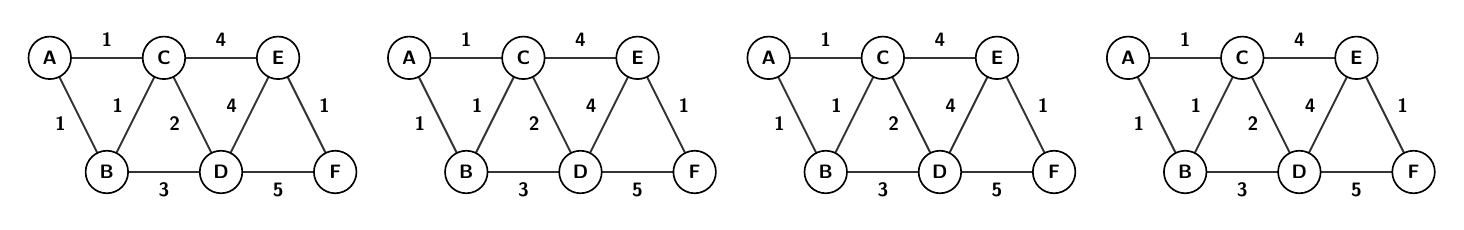
\begin{tikzpicture}[x=1mm,y=1mm]
\draw[line width=0.7pt, black!80] (2.70,18.32) -- (9.95,3.82);
\draw[line width=0.7pt, black!80] (2.70,18.32) -- (17.20,18.32);
\draw[line width=0.7pt, black!80] (9.95,3.82) -- (17.20,18.32);
\draw[line width=0.7pt, black!80] (17.20,18.32) -- (24.45,3.82);
\draw[line width=0.7pt, black!80] (9.95,3.82) -- (24.45,3.82);
\draw[line width=0.7pt, black!80] (17.20,18.32) -- (31.70,18.32);
\draw[line width=0.7pt, black!80] (24.45,3.82) -- (31.70,18.32);
\draw[line width=0.7pt, black!80] (31.70,18.32) -- (38.95,3.82);
\draw[line width=0.7pt, black!80] (24.45,3.82) -- (38.95,3.82);
\node[fill=white, inner sep=0, minimum width=2.30mm, minimum height=3.00mm, font=\scriptsize\bfseries] at (4.07,9.95) {1};
\node[fill=white, inner sep=0, minimum width=2.30mm, minimum height=3.00mm, font=\scriptsize\bfseries] at (9.95,20.65) {1};
\node[fill=white, inner sep=0, minimum width=2.30mm, minimum height=3.00mm, font=\scriptsize\bfseries] at (11.32,12.20) {1};
\node[fill=white, inner sep=0, minimum width=2.30mm, minimum height=3.00mm, font=\scriptsize\bfseries] at (18.57,9.95) {2};
\node[fill=white, inner sep=0, minimum width=2.30mm, minimum height=3.00mm, font=\scriptsize\bfseries] at (17.20,1.50) {3};
\node[fill=white, inner sep=0, minimum width=2.30mm, minimum height=3.00mm, font=\scriptsize\bfseries] at (24.45,20.65) {4};
\node[fill=white, inner sep=0, minimum width=2.30mm, minimum height=3.00mm, font=\scriptsize\bfseries] at (25.82,12.20) {4};
\node[fill=white, inner sep=0, minimum width=2.30mm, minimum height=3.00mm, font=\scriptsize\bfseries] at (37.58,12.20) {1};
\node[fill=white, inner sep=0, minimum width=2.30mm, minimum height=3.00mm, font=\scriptsize\bfseries] at (31.70,1.50) {5};
\node[circle, draw, line width=0.6pt, fill=white, minimum size=5.40mm, inner sep=0, font=\scriptsize\bfseries] at (2.70,18.32) {A};
\node[circle, draw, line width=0.6pt, fill=white, minimum size=5.40mm, inner sep=0, font=\scriptsize\bfseries] at (17.20,18.32) {C};
\node[circle, draw, line width=0.6pt, fill=white, minimum size=5.40mm, inner sep=0, font=\scriptsize\bfseries] at (31.70,18.32) {E};
\node[circle, draw, line width=0.6pt, fill=white, minimum size=5.40mm, inner sep=0, font=\scriptsize\bfseries] at (9.95,3.82) {B};
\node[circle, draw, line width=0.6pt, fill=white, minimum size=5.40mm, inner sep=0, font=\scriptsize\bfseries] at (24.45,3.82) {D};
\node[circle, draw, line width=0.6pt, fill=white, minimum size=5.40mm, inner sep=0, font=\scriptsize\bfseries] at (38.95,3.82) {F};
\draw[line width=0.7pt, black!80] (48.35,18.32) -- (55.60,3.82);
\draw[line width=0.7pt, black!80] (48.35,18.32) -- (62.85,18.32);
\draw[line width=0.7pt, black!80] (55.60,3.82) -- (62.85,18.32);
\draw[line width=0.7pt, black!80] (62.85,18.32) -- (70.10,3.82);
\draw[line width=0.7pt, black!80] (55.60,3.82) -- (70.10,3.82);
\draw[line width=0.7pt, black!80] (62.85,18.32) -- (77.35,18.32);
\draw[line width=0.7pt, black!80] (70.10,3.82) -- (77.35,18.32);
\draw[line width=0.7pt, black!80] (77.35,18.32) -- (84.60,3.82);
\draw[line width=0.7pt, black!80] (70.10,3.82) -- (84.60,3.82);
\node[fill=white, inner sep=0, minimum width=2.30mm, minimum height=3.00mm, font=\scriptsize\bfseries] at (49.72,9.95) {1};
\node[fill=white, inner sep=0, minimum width=2.30mm, minimum height=3.00mm, font=\scriptsize\bfseries] at (55.60,20.65) {1};
\node[fill=white, inner sep=0, minimum width=2.30mm, minimum height=3.00mm, font=\scriptsize\bfseries] at (56.97,12.20) {1};
\node[fill=white, inner sep=0, minimum width=2.30mm, minimum height=3.00mm, font=\scriptsize\bfseries] at (64.22,9.95) {2};
\node[fill=white, inner sep=0, minimum width=2.30mm, minimum height=3.00mm, font=\scriptsize\bfseries] at (62.85,1.50) {3};
\node[fill=white, inner sep=0, minimum width=2.30mm, minimum height=3.00mm, font=\scriptsize\bfseries] at (70.10,20.65) {4};
\node[fill=white, inner sep=0, minimum width=2.30mm, minimum height=3.00mm, font=\scriptsize\bfseries] at (71.47,12.20) {4};
\node[fill=white, inner sep=0, minimum width=2.30mm, minimum height=3.00mm, font=\scriptsize\bfseries] at (83.23,12.20) {1};
\node[fill=white, inner sep=0, minimum width=2.30mm, minimum height=3.00mm, font=\scriptsize\bfseries] at (77.35,1.50) {5};
\node[circle, draw, line width=0.6pt, fill=white, minimum size=5.40mm, inner sep=0, font=\scriptsize\bfseries] at (48.35,18.32) {A};
\node[circle, draw, line width=0.6pt, fill=white, minimum size=5.40mm, inner sep=0, font=\scriptsize\bfseries] at (62.85,18.32) {C};
\node[circle, draw, line width=0.6pt, fill=white, minimum size=5.40mm, inner sep=0, font=\scriptsize\bfseries] at (77.35,18.32) {E};
\node[circle, draw, line width=0.6pt, fill=white, minimum size=5.40mm, inner sep=0, font=\scriptsize\bfseries] at (55.60,3.82) {B};
\node[circle, draw, line width=0.6pt, fill=white, minimum size=5.40mm, inner sep=0, font=\scriptsize\bfseries] at (70.10,3.82) {D};
\node[circle, draw, line width=0.6pt, fill=white, minimum size=5.40mm, inner sep=0, font=\scriptsize\bfseries] at (84.60,3.82) {F};
\draw[line width=0.7pt, black!80] (94.00,18.32) -- (101.25,3.82);
\draw[line width=0.7pt, black!80] (94.00,18.32) -- (108.50,18.32);
\draw[line width=0.7pt, black!80] (101.25,3.82) -- (108.50,18.32);
\draw[line width=0.7pt, black!80] (108.50,18.32) -- (115.75,3.82);
\draw[line width=0.7pt, black!80] (101.25,3.82) -- (115.75,3.82);
\draw[line width=0.7pt, black!80] (108.50,18.32) -- (123.00,18.32);
\draw[line width=0.7pt, black!80] (115.75,3.82) -- (123.00,18.32);
\draw[line width=0.7pt, black!80] (123.00,18.32) -- (130.25,3.82);
\draw[line width=0.7pt, black!80] (115.75,3.82) -- (130.25,3.82);
\node[fill=white, inner sep=0, minimum width=2.30mm, minimum height=3.00mm, font=\scriptsize\bfseries] at (95.37,9.95) {1};
\node[fill=white, inner sep=0, minimum width=2.30mm, minimum height=3.00mm, font=\scriptsize\bfseries] at (101.25,20.65) {1};
\node[fill=white, inner sep=0, minimum width=2.30mm, minimum height=3.00mm, font=\scriptsize\bfseries] at (102.62,12.20) {1};
\node[fill=white, inner sep=0, minimum width=2.30mm, minimum height=3.00mm, font=\scriptsize\bfseries] at (109.87,9.95) {2};
\node[fill=white, inner sep=0, minimum width=2.30mm, minimum height=3.00mm, font=\scriptsize\bfseries] at (108.50,1.50) {3};
\node[fill=white, inner sep=0, minimum width=2.30mm, minimum height=3.00mm, font=\scriptsize\bfseries] at (115.75,20.65) {4};
\node[fill=white, inner sep=0, minimum width=2.30mm, minimum height=3.00mm, font=\scriptsize\bfseries] at (117.12,12.20) {4};
\node[fill=white, inner sep=0, minimum width=2.30mm, minimum height=3.00mm, font=\scriptsize\bfseries] at (128.88,12.20) {1};
\node[fill=white, inner sep=0, minimum width=2.30mm, minimum height=3.00mm, font=\scriptsize\bfseries] at (123.00,1.50) {5};
\node[circle, draw, line width=0.6pt, fill=white, minimum size=5.40mm, inner sep=0, font=\scriptsize\bfseries] at (94.00,18.32) {A};
\node[circle, draw, line width=0.6pt, fill=white, minimum size=5.40mm, inner sep=0, font=\scriptsize\bfseries] at (108.50,18.32) {C};
\node[circle, draw, line width=0.6pt, fill=white, minimum size=5.40mm, inner sep=0, font=\scriptsize\bfseries] at (123.00,18.32) {E};
\node[circle, draw, line width=0.6pt, fill=white, minimum size=5.40mm, inner sep=0, font=\scriptsize\bfseries] at (101.25,3.82) {B};
\node[circle, draw, line width=0.6pt, fill=white, minimum size=5.40mm, inner sep=0, font=\scriptsize\bfseries] at (115.75,3.82) {D};
\node[circle, draw, line width=0.6pt, fill=white, minimum size=5.40mm, inner sep=0, font=\scriptsize\bfseries] at (130.25,3.82) {F};
\draw[line width=0.7pt, black!80] (139.65,18.32) -- (146.90,3.82);
\draw[line width=0.7pt, black!80] (139.65,18.32) -- (154.15,18.32);
\draw[line width=0.7pt, black!80] (146.90,3.82) -- (154.15,18.32);
\draw[line width=0.7pt, black!80] (154.15,18.32) -- (161.40,3.82);
\draw[line width=0.7pt, black!80] (146.90,3.82) -- (161.40,3.82);
\draw[line width=0.7pt, black!80] (154.15,18.32) -- (168.65,18.32);
\draw[line width=0.7pt, black!80] (161.40,3.82) -- (168.65,18.32);
\draw[line width=0.7pt, black!80] (168.65,18.32) -- (175.90,3.82);
\draw[line width=0.7pt, black!80] (161.40,3.82) -- (175.90,3.82);
\node[fill=white, inner sep=0, minimum width=2.30mm, minimum height=3.00mm, font=\scriptsize\bfseries] at (141.02,9.95) {1};
\node[fill=white, inner sep=0, minimum width=2.30mm, minimum height=3.00mm, font=\scriptsize\bfseries] at (146.90,20.65) {1};
\node[fill=white, inner sep=0, minimum width=2.30mm, minimum height=3.00mm, font=\scriptsize\bfseries] at (148.27,12.20) {1};
\node[fill=white, inner sep=0, minimum width=2.30mm, minimum height=3.00mm, font=\scriptsize\bfseries] at (155.52,9.95) {2};
\node[fill=white, inner sep=0, minimum width=2.30mm, minimum height=3.00mm, font=\scriptsize\bfseries] at (154.15,1.50) {3};
\node[fill=white, inner sep=0, minimum width=2.30mm, minimum height=3.00mm, font=\scriptsize\bfseries] at (161.40,20.65) {4};
\node[fill=white, inner sep=0, minimum width=2.30mm, minimum height=3.00mm, font=\scriptsize\bfseries] at (162.77,12.20) {4};
\node[fill=white, inner sep=0, minimum width=2.30mm, minimum height=3.00mm, font=\scriptsize\bfseries] at (174.53,12.20) {1};
\node[fill=white, inner sep=0, minimum width=2.30mm, minimum height=3.00mm, font=\scriptsize\bfseries] at (168.65,1.50) {5};
\node[circle, draw, line width=0.6pt, fill=white, minimum size=5.40mm, inner sep=0, font=\scriptsize\bfseries] at (139.65,18.32) {A};
\node[circle, draw, line width=0.6pt, fill=white, minimum size=5.40mm, inner sep=0, font=\scriptsize\bfseries] at (154.15,18.32) {C};
\node[circle, draw, line width=0.6pt, fill=white, minimum size=5.40mm, inner sep=0, font=\scriptsize\bfseries] at (168.65,18.32) {E};
\node[circle, draw, line width=0.6pt, fill=white, minimum size=5.40mm, inner sep=0, font=\scriptsize\bfseries] at (146.90,3.82) {B};
\node[circle, draw, line width=0.6pt, fill=white, minimum size=5.40mm, inner sep=0, font=\scriptsize\bfseries] at (161.40,3.82) {D};
\node[circle, draw, line width=0.6pt, fill=white, minimum size=5.40mm, inner sep=0, font=\scriptsize\bfseries] at (175.90,3.82) {F};
\end{tikzpicture}
\end{center}\par

\vspace{-1mm}
\par\begin{center}
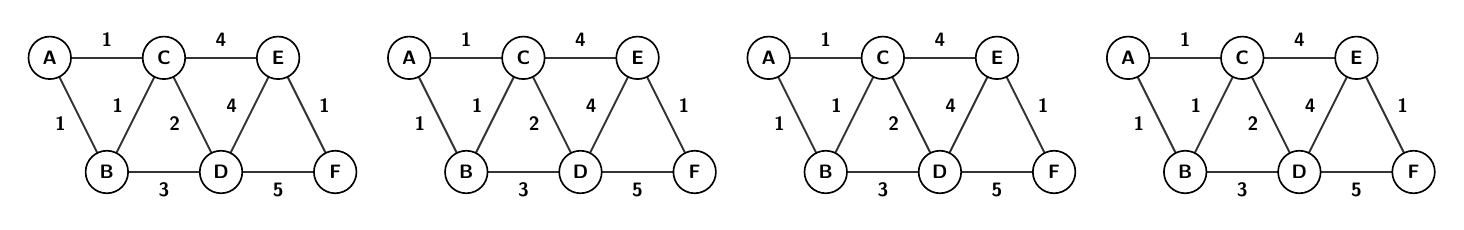
\begin{tikzpicture}[x=1mm,y=1mm]
\draw[line width=0.7pt, black!80] (2.70,18.32) -- (9.95,3.82);
\draw[line width=0.7pt, black!80] (2.70,18.32) -- (17.20,18.32);
\draw[line width=0.7pt, black!80] (9.95,3.82) -- (17.20,18.32);
\draw[line width=0.7pt, black!80] (17.20,18.32) -- (24.45,3.82);
\draw[line width=0.7pt, black!80] (9.95,3.82) -- (24.45,3.82);
\draw[line width=0.7pt, black!80] (17.20,18.32) -- (31.70,18.32);
\draw[line width=0.7pt, black!80] (24.45,3.82) -- (31.70,18.32);
\draw[line width=0.7pt, black!80] (31.70,18.32) -- (38.95,3.82);
\draw[line width=0.7pt, black!80] (24.45,3.82) -- (38.95,3.82);
\node[fill=white, inner sep=0, minimum width=2.30mm, minimum height=3.00mm, font=\scriptsize\bfseries] at (4.07,9.95) {1};
\node[fill=white, inner sep=0, minimum width=2.30mm, minimum height=3.00mm, font=\scriptsize\bfseries] at (9.95,20.65) {1};
\node[fill=white, inner sep=0, minimum width=2.30mm, minimum height=3.00mm, font=\scriptsize\bfseries] at (11.32,12.20) {1};
\node[fill=white, inner sep=0, minimum width=2.30mm, minimum height=3.00mm, font=\scriptsize\bfseries] at (18.57,9.95) {2};
\node[fill=white, inner sep=0, minimum width=2.30mm, minimum height=3.00mm, font=\scriptsize\bfseries] at (17.20,1.50) {3};
\node[fill=white, inner sep=0, minimum width=2.30mm, minimum height=3.00mm, font=\scriptsize\bfseries] at (24.45,20.65) {4};
\node[fill=white, inner sep=0, minimum width=2.30mm, minimum height=3.00mm, font=\scriptsize\bfseries] at (25.82,12.20) {4};
\node[fill=white, inner sep=0, minimum width=2.30mm, minimum height=3.00mm, font=\scriptsize\bfseries] at (37.58,12.20) {1};
\node[fill=white, inner sep=0, minimum width=2.30mm, minimum height=3.00mm, font=\scriptsize\bfseries] at (31.70,1.50) {5};
\node[circle, draw, line width=0.6pt, fill=white, minimum size=5.40mm, inner sep=0, font=\scriptsize\bfseries] at (2.70,18.32) {A};
\node[circle, draw, line width=0.6pt, fill=white, minimum size=5.40mm, inner sep=0, font=\scriptsize\bfseries] at (17.20,18.32) {C};
\node[circle, draw, line width=0.6pt, fill=white, minimum size=5.40mm, inner sep=0, font=\scriptsize\bfseries] at (31.70,18.32) {E};
\node[circle, draw, line width=0.6pt, fill=white, minimum size=5.40mm, inner sep=0, font=\scriptsize\bfseries] at (9.95,3.82) {B};
\node[circle, draw, line width=0.6pt, fill=white, minimum size=5.40mm, inner sep=0, font=\scriptsize\bfseries] at (24.45,3.82) {D};
\node[circle, draw, line width=0.6pt, fill=white, minimum size=5.40mm, inner sep=0, font=\scriptsize\bfseries] at (38.95,3.82) {F};
\draw[line width=0.7pt, black!80] (48.35,18.32) -- (55.60,3.82);
\draw[line width=0.7pt, black!80] (48.35,18.32) -- (62.85,18.32);
\draw[line width=0.7pt, black!80] (55.60,3.82) -- (62.85,18.32);
\draw[line width=0.7pt, black!80] (62.85,18.32) -- (70.10,3.82);
\draw[line width=0.7pt, black!80] (55.60,3.82) -- (70.10,3.82);
\draw[line width=0.7pt, black!80] (62.85,18.32) -- (77.35,18.32);
\draw[line width=0.7pt, black!80] (70.10,3.82) -- (77.35,18.32);
\draw[line width=0.7pt, black!80] (77.35,18.32) -- (84.60,3.82);
\draw[line width=0.7pt, black!80] (70.10,3.82) -- (84.60,3.82);
\node[fill=white, inner sep=0, minimum width=2.30mm, minimum height=3.00mm, font=\scriptsize\bfseries] at (49.72,9.95) {1};
\node[fill=white, inner sep=0, minimum width=2.30mm, minimum height=3.00mm, font=\scriptsize\bfseries] at (55.60,20.65) {1};
\node[fill=white, inner sep=0, minimum width=2.30mm, minimum height=3.00mm, font=\scriptsize\bfseries] at (56.97,12.20) {1};
\node[fill=white, inner sep=0, minimum width=2.30mm, minimum height=3.00mm, font=\scriptsize\bfseries] at (64.22,9.95) {2};
\node[fill=white, inner sep=0, minimum width=2.30mm, minimum height=3.00mm, font=\scriptsize\bfseries] at (62.85,1.50) {3};
\node[fill=white, inner sep=0, minimum width=2.30mm, minimum height=3.00mm, font=\scriptsize\bfseries] at (70.10,20.65) {4};
\node[fill=white, inner sep=0, minimum width=2.30mm, minimum height=3.00mm, font=\scriptsize\bfseries] at (71.47,12.20) {4};
\node[fill=white, inner sep=0, minimum width=2.30mm, minimum height=3.00mm, font=\scriptsize\bfseries] at (83.23,12.20) {1};
\node[fill=white, inner sep=0, minimum width=2.30mm, minimum height=3.00mm, font=\scriptsize\bfseries] at (77.35,1.50) {5};
\node[circle, draw, line width=0.6pt, fill=white, minimum size=5.40mm, inner sep=0, font=\scriptsize\bfseries] at (48.35,18.32) {A};
\node[circle, draw, line width=0.6pt, fill=white, minimum size=5.40mm, inner sep=0, font=\scriptsize\bfseries] at (62.85,18.32) {C};
\node[circle, draw, line width=0.6pt, fill=white, minimum size=5.40mm, inner sep=0, font=\scriptsize\bfseries] at (77.35,18.32) {E};
\node[circle, draw, line width=0.6pt, fill=white, minimum size=5.40mm, inner sep=0, font=\scriptsize\bfseries] at (55.60,3.82) {B};
\node[circle, draw, line width=0.6pt, fill=white, minimum size=5.40mm, inner sep=0, font=\scriptsize\bfseries] at (70.10,3.82) {D};
\node[circle, draw, line width=0.6pt, fill=white, minimum size=5.40mm, inner sep=0, font=\scriptsize\bfseries] at (84.60,3.82) {F};
\draw[line width=0.7pt, black!80] (94.00,18.32) -- (101.25,3.82);
\draw[line width=0.7pt, black!80] (94.00,18.32) -- (108.50,18.32);
\draw[line width=0.7pt, black!80] (101.25,3.82) -- (108.50,18.32);
\draw[line width=0.7pt, black!80] (108.50,18.32) -- (115.75,3.82);
\draw[line width=0.7pt, black!80] (101.25,3.82) -- (115.75,3.82);
\draw[line width=0.7pt, black!80] (108.50,18.32) -- (123.00,18.32);
\draw[line width=0.7pt, black!80] (115.75,3.82) -- (123.00,18.32);
\draw[line width=0.7pt, black!80] (123.00,18.32) -- (130.25,3.82);
\draw[line width=0.7pt, black!80] (115.75,3.82) -- (130.25,3.82);
\node[fill=white, inner sep=0, minimum width=2.30mm, minimum height=3.00mm, font=\scriptsize\bfseries] at (95.37,9.95) {1};
\node[fill=white, inner sep=0, minimum width=2.30mm, minimum height=3.00mm, font=\scriptsize\bfseries] at (101.25,20.65) {1};
\node[fill=white, inner sep=0, minimum width=2.30mm, minimum height=3.00mm, font=\scriptsize\bfseries] at (102.62,12.20) {1};
\node[fill=white, inner sep=0, minimum width=2.30mm, minimum height=3.00mm, font=\scriptsize\bfseries] at (109.87,9.95) {2};
\node[fill=white, inner sep=0, minimum width=2.30mm, minimum height=3.00mm, font=\scriptsize\bfseries] at (108.50,1.50) {3};
\node[fill=white, inner sep=0, minimum width=2.30mm, minimum height=3.00mm, font=\scriptsize\bfseries] at (115.75,20.65) {4};
\node[fill=white, inner sep=0, minimum width=2.30mm, minimum height=3.00mm, font=\scriptsize\bfseries] at (117.12,12.20) {4};
\node[fill=white, inner sep=0, minimum width=2.30mm, minimum height=3.00mm, font=\scriptsize\bfseries] at (128.88,12.20) {1};
\node[fill=white, inner sep=0, minimum width=2.30mm, minimum height=3.00mm, font=\scriptsize\bfseries] at (123.00,1.50) {5};
\node[circle, draw, line width=0.6pt, fill=white, minimum size=5.40mm, inner sep=0, font=\scriptsize\bfseries] at (94.00,18.32) {A};
\node[circle, draw, line width=0.6pt, fill=white, minimum size=5.40mm, inner sep=0, font=\scriptsize\bfseries] at (108.50,18.32) {C};
\node[circle, draw, line width=0.6pt, fill=white, minimum size=5.40mm, inner sep=0, font=\scriptsize\bfseries] at (123.00,18.32) {E};
\node[circle, draw, line width=0.6pt, fill=white, minimum size=5.40mm, inner sep=0, font=\scriptsize\bfseries] at (101.25,3.82) {B};
\node[circle, draw, line width=0.6pt, fill=white, minimum size=5.40mm, inner sep=0, font=\scriptsize\bfseries] at (115.75,3.82) {D};
\node[circle, draw, line width=0.6pt, fill=white, minimum size=5.40mm, inner sep=0, font=\scriptsize\bfseries] at (130.25,3.82) {F};
\draw[line width=0.7pt, black!80] (139.65,18.32) -- (146.90,3.82);
\draw[line width=0.7pt, black!80] (139.65,18.32) -- (154.15,18.32);
\draw[line width=0.7pt, black!80] (146.90,3.82) -- (154.15,18.32);
\draw[line width=0.7pt, black!80] (154.15,18.32) -- (161.40,3.82);
\draw[line width=0.7pt, black!80] (146.90,3.82) -- (161.40,3.82);
\draw[line width=0.7pt, black!80] (154.15,18.32) -- (168.65,18.32);
\draw[line width=0.7pt, black!80] (161.40,3.82) -- (168.65,18.32);
\draw[line width=0.7pt, black!80] (168.65,18.32) -- (175.90,3.82);
\draw[line width=0.7pt, black!80] (161.40,3.82) -- (175.90,3.82);
\node[fill=white, inner sep=0, minimum width=2.30mm, minimum height=3.00mm, font=\scriptsize\bfseries] at (141.02,9.95) {1};
\node[fill=white, inner sep=0, minimum width=2.30mm, minimum height=3.00mm, font=\scriptsize\bfseries] at (146.90,20.65) {1};
\node[fill=white, inner sep=0, minimum width=2.30mm, minimum height=3.00mm, font=\scriptsize\bfseries] at (148.27,12.20) {1};
\node[fill=white, inner sep=0, minimum width=2.30mm, minimum height=3.00mm, font=\scriptsize\bfseries] at (155.52,9.95) {2};
\node[fill=white, inner sep=0, minimum width=2.30mm, minimum height=3.00mm, font=\scriptsize\bfseries] at (154.15,1.50) {3};
\node[fill=white, inner sep=0, minimum width=2.30mm, minimum height=3.00mm, font=\scriptsize\bfseries] at (161.40,20.65) {4};
\node[fill=white, inner sep=0, minimum width=2.30mm, minimum height=3.00mm, font=\scriptsize\bfseries] at (162.77,12.20) {4};
\node[fill=white, inner sep=0, minimum width=2.30mm, minimum height=3.00mm, font=\scriptsize\bfseries] at (174.53,12.20) {1};
\node[fill=white, inner sep=0, minimum width=2.30mm, minimum height=3.00mm, font=\scriptsize\bfseries] at (168.65,1.50) {5};
\node[circle, draw, line width=0.6pt, fill=white, minimum size=5.40mm, inner sep=0, font=\scriptsize\bfseries] at (139.65,18.32) {A};
\node[circle, draw, line width=0.6pt, fill=white, minimum size=5.40mm, inner sep=0, font=\scriptsize\bfseries] at (154.15,18.32) {C};
\node[circle, draw, line width=0.6pt, fill=white, minimum size=5.40mm, inner sep=0, font=\scriptsize\bfseries] at (168.65,18.32) {E};
\node[circle, draw, line width=0.6pt, fill=white, minimum size=5.40mm, inner sep=0, font=\scriptsize\bfseries] at (146.90,3.82) {B};
\node[circle, draw, line width=0.6pt, fill=white, minimum size=5.40mm, inner sep=0, font=\scriptsize\bfseries] at (161.40,3.82) {D};
\node[circle, draw, line width=0.6pt, fill=white, minimum size=5.40mm, inner sep=0, font=\scriptsize\bfseries] at (175.90,3.82) {F};
\end{tikzpicture}
\end{center}\par

\newpage

\prob{3} On the big map, lay markers on the links priced 1, and draw a ring around each group of places that the pawn can walk between on markers, as in the small pictures. Then add the links priced 2, then 3, and so on, ringing the groups each time, until there is one group. At which price do A and D first share a ring? B and D? D and F? A and F?

\par\begin{center}
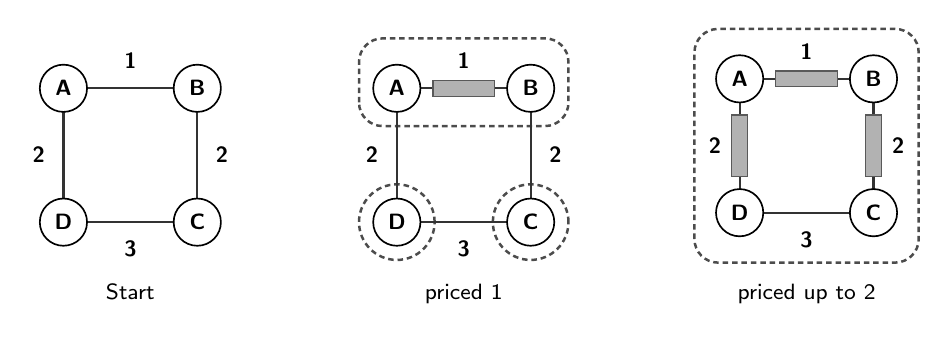
\begin{tikzpicture}[x=1mm,y=1mm]
\draw[line width=0.8pt, black!80] (4.54,27.14) -- (21.54,27.14);
\draw[line width=0.8pt, black!80] (21.54,27.14) -- (21.54,10.14);
\draw[line width=0.8pt, black!80] (21.54,10.14) -- (4.54,10.14);
\draw[line width=0.8pt, black!80] (4.54,10.14) -- (4.54,27.14);
\node[fill=white, inner sep=0, minimum width=2.80mm, minimum height=3.40mm, font=\footnotesize\bfseries] at (13.04,30.58) {1};
\node[fill=white, inner sep=0, minimum width=2.80mm, minimum height=3.40mm, font=\footnotesize\bfseries] at (24.68,18.64) {2};
\node[fill=white, inner sep=0, minimum width=2.80mm, minimum height=3.40mm, font=\footnotesize\bfseries] at (13.04,6.70) {3};
\node[fill=white, inner sep=0, minimum width=2.80mm, minimum height=3.40mm, font=\footnotesize\bfseries] at (1.40,18.64) {2};
\node[circle, draw, line width=0.6pt, fill=white, minimum size=6.00mm, inner sep=0, font=\footnotesize\bfseries] at (4.54,27.14) {A};
\node[circle, draw, line width=0.6pt, fill=white, minimum size=6.00mm, inner sep=0, font=\footnotesize\bfseries] at (21.54,27.14) {B};
\node[circle, draw, line width=0.6pt, fill=white, minimum size=6.00mm, inner sep=0, font=\footnotesize\bfseries] at (21.54,10.14) {C};
\node[circle, draw, line width=0.6pt, fill=white, minimum size=6.00mm, inner sep=0, font=\footnotesize\bfseries] at (4.54,10.14) {D};
\node[font=\footnotesize, anchor=north, align=center] at (13.04,3.50) {Start};
\draw[black!70, line width=0.9pt, dash pattern=on 2pt off 1.4pt, rounded corners=3mm] (42.08,22.34) rectangle (68.68,33.48);
\draw[black!70, line width=0.9pt, dash pattern=on 2pt off 1.4pt] (63.88,10.14) circle (4.80mm);
\draw[black!70, line width=0.9pt, dash pattern=on 2pt off 1.4pt] (46.88,10.14) circle (4.80mm);
\draw[line width=0.8pt, black!80] (46.88,27.14) -- (63.88,27.14);
\draw[line width=0.8pt, black!80] (63.88,27.14) -- (63.88,10.14);
\draw[line width=0.8pt, black!80] (63.88,10.14) -- (46.88,10.14);
\draw[line width=0.8pt, black!80] (46.88,10.14) -- (46.88,27.14);
\filldraw[fill=black!30, draw=black!65, line width=0.4pt] (51.47,28.14) -- (59.29,28.14) -- (59.29,26.14) -- (51.47,26.14) -- cycle;
\node[fill=white, inner sep=0, minimum width=2.80mm, minimum height=3.40mm, font=\footnotesize\bfseries] at (55.38,30.58) {1};
\node[fill=white, inner sep=0, minimum width=2.80mm, minimum height=3.40mm, font=\footnotesize\bfseries] at (67.02,18.64) {2};
\node[fill=white, inner sep=0, minimum width=2.80mm, minimum height=3.40mm, font=\footnotesize\bfseries] at (55.38,6.70) {3};
\node[fill=white, inner sep=0, minimum width=2.80mm, minimum height=3.40mm, font=\footnotesize\bfseries] at (43.74,18.64) {2};
\node[circle, draw, line width=0.6pt, fill=white, minimum size=6.00mm, inner sep=0, font=\footnotesize\bfseries] at (46.88,27.14) {A};
\node[circle, draw, line width=0.6pt, fill=white, minimum size=6.00mm, inner sep=0, font=\footnotesize\bfseries] at (63.88,27.14) {B};
\node[circle, draw, line width=0.6pt, fill=white, minimum size=6.00mm, inner sep=0, font=\footnotesize\bfseries] at (63.88,10.14) {C};
\node[circle, draw, line width=0.6pt, fill=white, minimum size=6.00mm, inner sep=0, font=\footnotesize\bfseries] at (46.88,10.14) {D};
\node[font=\footnotesize, anchor=north, align=center] at (55.38,3.50) {priced 1};
\draw[black!70, line width=0.9pt, dash pattern=on 2pt off 1.4pt, rounded corners=3mm] (84.68,5.00) rectangle (113.16,34.68);
\draw[line width=0.8pt, black!80] (90.42,28.34) -- (107.42,28.34);
\draw[line width=0.8pt, black!80] (107.42,28.34) -- (107.42,11.34);
\draw[line width=0.8pt, black!80] (107.42,11.34) -- (90.42,11.34);
\draw[line width=0.8pt, black!80] (90.42,11.34) -- (90.42,28.34);
\filldraw[fill=black!30, draw=black!65, line width=0.4pt] (95.01,29.34) -- (102.83,29.34) -- (102.83,27.34) -- (95.01,27.34) -- cycle;
\filldraw[fill=black!30, draw=black!65, line width=0.4pt] (108.42,23.75) -- (108.42,15.93) -- (106.42,15.93) -- (106.42,23.75) -- cycle;
\filldraw[fill=black!30, draw=black!65, line width=0.4pt] (89.42,15.93) -- (89.42,23.75) -- (91.42,23.75) -- (91.42,15.93) -- cycle;
\node[fill=white, inner sep=0, minimum width=2.80mm, minimum height=3.40mm, font=\footnotesize\bfseries] at (98.92,31.78) {1};
\node[fill=white, inner sep=0, minimum width=2.80mm, minimum height=3.40mm, font=\footnotesize\bfseries] at (110.56,19.84) {2};
\node[fill=white, inner sep=0, minimum width=2.80mm, minimum height=3.40mm, font=\footnotesize\bfseries] at (98.92,7.90) {3};
\node[fill=white, inner sep=0, minimum width=2.80mm, minimum height=3.40mm, font=\footnotesize\bfseries] at (87.28,19.84) {2};
\node[circle, draw, line width=0.6pt, fill=white, minimum size=6.00mm, inner sep=0, font=\footnotesize\bfseries] at (90.42,28.34) {A};
\node[circle, draw, line width=0.6pt, fill=white, minimum size=6.00mm, inner sep=0, font=\footnotesize\bfseries] at (107.42,28.34) {B};
\node[circle, draw, line width=0.6pt, fill=white, minimum size=6.00mm, inner sep=0, font=\footnotesize\bfseries] at (107.42,11.34) {C};
\node[circle, draw, line width=0.6pt, fill=white, minimum size=6.00mm, inner sep=0, font=\footnotesize\bfseries] at (90.42,11.34) {D};
\node[font=\footnotesize, anchor=north, align=center] at (98.92,3.50) {priced up to 2};
\end{tikzpicture}
\end{center}\par

\par\begin{center}
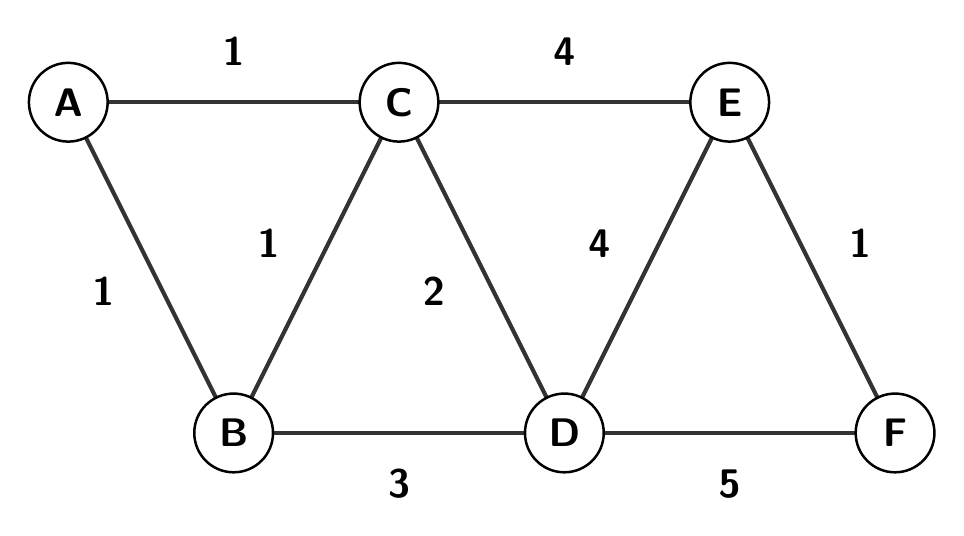
\begin{tikzpicture}[x=1mm,y=1mm]
\draw[line width=1.5pt, black!80] (5.00,51.46) -- (26.00,9.46);
\draw[line width=1.5pt, black!80] (5.00,51.46) -- (47.00,51.46);
\draw[line width=1.5pt, black!80] (26.00,9.46) -- (47.00,51.46);
\draw[line width=1.5pt, black!80] (47.00,51.46) -- (68.00,9.46);
\draw[line width=1.5pt, black!80] (26.00,9.46) -- (68.00,9.46);
\draw[line width=1.5pt, black!80] (47.00,51.46) -- (89.00,51.46);
\draw[line width=1.5pt, black!80] (68.00,9.46) -- (89.00,51.46);
\draw[line width=1.5pt, black!80] (89.00,51.46) -- (110.00,9.46);
\draw[line width=1.5pt, black!80] (68.00,9.46) -- (110.00,9.46);
\node[fill=white, inner sep=0, minimum width=4.40mm, minimum height=6.00mm, font=\Large\bfseries] at (9.44,27.44) {1};
\node[fill=white, inner sep=0, minimum width=4.40mm, minimum height=6.00mm, font=\Large\bfseries] at (26.00,57.93) {1};
\node[fill=white, inner sep=0, minimum width=4.40mm, minimum height=6.00mm, font=\Large\bfseries] at (30.44,33.49) {1};
\node[fill=white, inner sep=0, minimum width=4.40mm, minimum height=6.00mm, font=\Large\bfseries] at (51.44,27.44) {2};
\node[fill=white, inner sep=0, minimum width=4.40mm, minimum height=6.00mm, font=\Large\bfseries] at (47.00,3.00) {3};
\node[fill=white, inner sep=0, minimum width=4.40mm, minimum height=6.00mm, font=\Large\bfseries] at (68.00,57.93) {4};
\node[fill=white, inner sep=0, minimum width=4.40mm, minimum height=6.00mm, font=\Large\bfseries] at (72.44,33.49) {4};
\node[fill=white, inner sep=0, minimum width=4.40mm, minimum height=6.00mm, font=\Large\bfseries] at (105.56,33.49) {1};
\node[fill=white, inner sep=0, minimum width=4.40mm, minimum height=6.00mm, font=\Large\bfseries] at (89.00,3.00) {5};
\node[circle, draw, line width=0.9pt, fill=white, minimum size=10.00mm, inner sep=0, font=\Large\bfseries] at (5.00,51.46) {A};
\node[circle, draw, line width=0.9pt, fill=white, minimum size=10.00mm, inner sep=0, font=\Large\bfseries] at (47.00,51.46) {C};
\node[circle, draw, line width=0.9pt, fill=white, minimum size=10.00mm, inner sep=0, font=\Large\bfseries] at (89.00,51.46) {E};
\node[circle, draw, line width=0.9pt, fill=white, minimum size=10.00mm, inner sep=0, font=\Large\bfseries] at (26.00,9.46) {B};
\node[circle, draw, line width=0.9pt, fill=white, minimum size=10.00mm, inner sep=0, font=\Large\bfseries] at (68.00,9.46) {D};
\node[circle, draw, line width=0.9pt, fill=white, minimum size=10.00mm, inner sep=0, font=\Large\bfseries] at (110.00,9.46) {F};
\end{tikzpicture}
\end{center}\par

\par\begin{center}
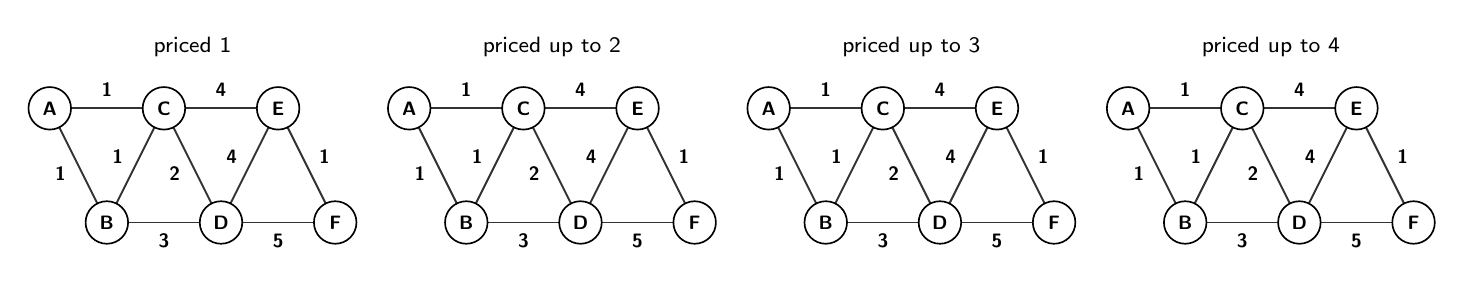
\begin{tikzpicture}[x=1mm,y=1mm]
\draw[line width=0.7pt, black!80] (2.70,18.32) -- (9.95,3.82);
\draw[line width=0.7pt, black!80] (2.70,18.32) -- (17.20,18.32);
\draw[line width=0.7pt, black!80] (9.95,3.82) -- (17.20,18.32);
\draw[line width=0.7pt, black!80] (17.20,18.32) -- (24.45,3.82);
\draw[line width=0.7pt, black!80] (9.95,3.82) -- (24.45,3.82);
\draw[line width=0.7pt, black!80] (17.20,18.32) -- (31.70,18.32);
\draw[line width=0.7pt, black!80] (24.45,3.82) -- (31.70,18.32);
\draw[line width=0.7pt, black!80] (31.70,18.32) -- (38.95,3.82);
\draw[line width=0.7pt, black!80] (24.45,3.82) -- (38.95,3.82);
\node[fill=white, inner sep=0, minimum width=2.30mm, minimum height=3.00mm, font=\scriptsize\bfseries] at (4.07,9.95) {1};
\node[fill=white, inner sep=0, minimum width=2.30mm, minimum height=3.00mm, font=\scriptsize\bfseries] at (9.95,20.65) {1};
\node[fill=white, inner sep=0, minimum width=2.30mm, minimum height=3.00mm, font=\scriptsize\bfseries] at (11.32,12.20) {1};
\node[fill=white, inner sep=0, minimum width=2.30mm, minimum height=3.00mm, font=\scriptsize\bfseries] at (18.57,9.95) {2};
\node[fill=white, inner sep=0, minimum width=2.30mm, minimum height=3.00mm, font=\scriptsize\bfseries] at (17.20,1.50) {3};
\node[fill=white, inner sep=0, minimum width=2.30mm, minimum height=3.00mm, font=\scriptsize\bfseries] at (24.45,20.65) {4};
\node[fill=white, inner sep=0, minimum width=2.30mm, minimum height=3.00mm, font=\scriptsize\bfseries] at (25.82,12.20) {4};
\node[fill=white, inner sep=0, minimum width=2.30mm, minimum height=3.00mm, font=\scriptsize\bfseries] at (37.58,12.20) {1};
\node[fill=white, inner sep=0, minimum width=2.30mm, minimum height=3.00mm, font=\scriptsize\bfseries] at (31.70,1.50) {5};
\node[circle, draw, line width=0.6pt, fill=white, minimum size=5.40mm, inner sep=0, font=\scriptsize\bfseries] at (2.70,18.32) {A};
\node[circle, draw, line width=0.6pt, fill=white, minimum size=5.40mm, inner sep=0, font=\scriptsize\bfseries] at (17.20,18.32) {C};
\node[circle, draw, line width=0.6pt, fill=white, minimum size=5.40mm, inner sep=0, font=\scriptsize\bfseries] at (31.70,18.32) {E};
\node[circle, draw, line width=0.6pt, fill=white, minimum size=5.40mm, inner sep=0, font=\scriptsize\bfseries] at (9.95,3.82) {B};
\node[circle, draw, line width=0.6pt, fill=white, minimum size=5.40mm, inner sep=0, font=\scriptsize\bfseries] at (24.45,3.82) {D};
\node[circle, draw, line width=0.6pt, fill=white, minimum size=5.40mm, inner sep=0, font=\scriptsize\bfseries] at (38.95,3.82) {F};
\node[font=\footnotesize, anchor=south, align=center] at (20.83,23.65) {priced 1};
\draw[line width=0.7pt, black!80] (48.35,18.32) -- (55.60,3.82);
\draw[line width=0.7pt, black!80] (48.35,18.32) -- (62.85,18.32);
\draw[line width=0.7pt, black!80] (55.60,3.82) -- (62.85,18.32);
\draw[line width=0.7pt, black!80] (62.85,18.32) -- (70.10,3.82);
\draw[line width=0.7pt, black!80] (55.60,3.82) -- (70.10,3.82);
\draw[line width=0.7pt, black!80] (62.85,18.32) -- (77.35,18.32);
\draw[line width=0.7pt, black!80] (70.10,3.82) -- (77.35,18.32);
\draw[line width=0.7pt, black!80] (77.35,18.32) -- (84.60,3.82);
\draw[line width=0.7pt, black!80] (70.10,3.82) -- (84.60,3.82);
\node[fill=white, inner sep=0, minimum width=2.30mm, minimum height=3.00mm, font=\scriptsize\bfseries] at (49.72,9.95) {1};
\node[fill=white, inner sep=0, minimum width=2.30mm, minimum height=3.00mm, font=\scriptsize\bfseries] at (55.60,20.65) {1};
\node[fill=white, inner sep=0, minimum width=2.30mm, minimum height=3.00mm, font=\scriptsize\bfseries] at (56.97,12.20) {1};
\node[fill=white, inner sep=0, minimum width=2.30mm, minimum height=3.00mm, font=\scriptsize\bfseries] at (64.22,9.95) {2};
\node[fill=white, inner sep=0, minimum width=2.30mm, minimum height=3.00mm, font=\scriptsize\bfseries] at (62.85,1.50) {3};
\node[fill=white, inner sep=0, minimum width=2.30mm, minimum height=3.00mm, font=\scriptsize\bfseries] at (70.10,20.65) {4};
\node[fill=white, inner sep=0, minimum width=2.30mm, minimum height=3.00mm, font=\scriptsize\bfseries] at (71.47,12.20) {4};
\node[fill=white, inner sep=0, minimum width=2.30mm, minimum height=3.00mm, font=\scriptsize\bfseries] at (83.23,12.20) {1};
\node[fill=white, inner sep=0, minimum width=2.30mm, minimum height=3.00mm, font=\scriptsize\bfseries] at (77.35,1.50) {5};
\node[circle, draw, line width=0.6pt, fill=white, minimum size=5.40mm, inner sep=0, font=\scriptsize\bfseries] at (48.35,18.32) {A};
\node[circle, draw, line width=0.6pt, fill=white, minimum size=5.40mm, inner sep=0, font=\scriptsize\bfseries] at (62.85,18.32) {C};
\node[circle, draw, line width=0.6pt, fill=white, minimum size=5.40mm, inner sep=0, font=\scriptsize\bfseries] at (77.35,18.32) {E};
\node[circle, draw, line width=0.6pt, fill=white, minimum size=5.40mm, inner sep=0, font=\scriptsize\bfseries] at (55.60,3.82) {B};
\node[circle, draw, line width=0.6pt, fill=white, minimum size=5.40mm, inner sep=0, font=\scriptsize\bfseries] at (70.10,3.82) {D};
\node[circle, draw, line width=0.6pt, fill=white, minimum size=5.40mm, inner sep=0, font=\scriptsize\bfseries] at (84.60,3.82) {F};
\node[font=\footnotesize, anchor=south, align=center] at (66.48,23.65) {priced up to 2};
\draw[line width=0.7pt, black!80] (94.00,18.32) -- (101.25,3.82);
\draw[line width=0.7pt, black!80] (94.00,18.32) -- (108.50,18.32);
\draw[line width=0.7pt, black!80] (101.25,3.82) -- (108.50,18.32);
\draw[line width=0.7pt, black!80] (108.50,18.32) -- (115.75,3.82);
\draw[line width=0.7pt, black!80] (101.25,3.82) -- (115.75,3.82);
\draw[line width=0.7pt, black!80] (108.50,18.32) -- (123.00,18.32);
\draw[line width=0.7pt, black!80] (115.75,3.82) -- (123.00,18.32);
\draw[line width=0.7pt, black!80] (123.00,18.32) -- (130.25,3.82);
\draw[line width=0.7pt, black!80] (115.75,3.82) -- (130.25,3.82);
\node[fill=white, inner sep=0, minimum width=2.30mm, minimum height=3.00mm, font=\scriptsize\bfseries] at (95.37,9.95) {1};
\node[fill=white, inner sep=0, minimum width=2.30mm, minimum height=3.00mm, font=\scriptsize\bfseries] at (101.25,20.65) {1};
\node[fill=white, inner sep=0, minimum width=2.30mm, minimum height=3.00mm, font=\scriptsize\bfseries] at (102.62,12.20) {1};
\node[fill=white, inner sep=0, minimum width=2.30mm, minimum height=3.00mm, font=\scriptsize\bfseries] at (109.87,9.95) {2};
\node[fill=white, inner sep=0, minimum width=2.30mm, minimum height=3.00mm, font=\scriptsize\bfseries] at (108.50,1.50) {3};
\node[fill=white, inner sep=0, minimum width=2.30mm, minimum height=3.00mm, font=\scriptsize\bfseries] at (115.75,20.65) {4};
\node[fill=white, inner sep=0, minimum width=2.30mm, minimum height=3.00mm, font=\scriptsize\bfseries] at (117.12,12.20) {4};
\node[fill=white, inner sep=0, minimum width=2.30mm, minimum height=3.00mm, font=\scriptsize\bfseries] at (128.88,12.20) {1};
\node[fill=white, inner sep=0, minimum width=2.30mm, minimum height=3.00mm, font=\scriptsize\bfseries] at (123.00,1.50) {5};
\node[circle, draw, line width=0.6pt, fill=white, minimum size=5.40mm, inner sep=0, font=\scriptsize\bfseries] at (94.00,18.32) {A};
\node[circle, draw, line width=0.6pt, fill=white, minimum size=5.40mm, inner sep=0, font=\scriptsize\bfseries] at (108.50,18.32) {C};
\node[circle, draw, line width=0.6pt, fill=white, minimum size=5.40mm, inner sep=0, font=\scriptsize\bfseries] at (123.00,18.32) {E};
\node[circle, draw, line width=0.6pt, fill=white, minimum size=5.40mm, inner sep=0, font=\scriptsize\bfseries] at (101.25,3.82) {B};
\node[circle, draw, line width=0.6pt, fill=white, minimum size=5.40mm, inner sep=0, font=\scriptsize\bfseries] at (115.75,3.82) {D};
\node[circle, draw, line width=0.6pt, fill=white, minimum size=5.40mm, inner sep=0, font=\scriptsize\bfseries] at (130.25,3.82) {F};
\node[font=\footnotesize, anchor=south, align=center] at (112.13,23.65) {priced up to 3};
\draw[line width=0.7pt, black!80] (139.65,18.32) -- (146.90,3.82);
\draw[line width=0.7pt, black!80] (139.65,18.32) -- (154.15,18.32);
\draw[line width=0.7pt, black!80] (146.90,3.82) -- (154.15,18.32);
\draw[line width=0.7pt, black!80] (154.15,18.32) -- (161.40,3.82);
\draw[line width=0.7pt, black!80] (146.90,3.82) -- (161.40,3.82);
\draw[line width=0.7pt, black!80] (154.15,18.32) -- (168.65,18.32);
\draw[line width=0.7pt, black!80] (161.40,3.82) -- (168.65,18.32);
\draw[line width=0.7pt, black!80] (168.65,18.32) -- (175.90,3.82);
\draw[line width=0.7pt, black!80] (161.40,3.82) -- (175.90,3.82);
\node[fill=white, inner sep=0, minimum width=2.30mm, minimum height=3.00mm, font=\scriptsize\bfseries] at (141.02,9.95) {1};
\node[fill=white, inner sep=0, minimum width=2.30mm, minimum height=3.00mm, font=\scriptsize\bfseries] at (146.90,20.65) {1};
\node[fill=white, inner sep=0, minimum width=2.30mm, minimum height=3.00mm, font=\scriptsize\bfseries] at (148.27,12.20) {1};
\node[fill=white, inner sep=0, minimum width=2.30mm, minimum height=3.00mm, font=\scriptsize\bfseries] at (155.52,9.95) {2};
\node[fill=white, inner sep=0, minimum width=2.30mm, minimum height=3.00mm, font=\scriptsize\bfseries] at (154.15,1.50) {3};
\node[fill=white, inner sep=0, minimum width=2.30mm, minimum height=3.00mm, font=\scriptsize\bfseries] at (161.40,20.65) {4};
\node[fill=white, inner sep=0, minimum width=2.30mm, minimum height=3.00mm, font=\scriptsize\bfseries] at (162.77,12.20) {4};
\node[fill=white, inner sep=0, minimum width=2.30mm, minimum height=3.00mm, font=\scriptsize\bfseries] at (174.53,12.20) {1};
\node[fill=white, inner sep=0, minimum width=2.30mm, minimum height=3.00mm, font=\scriptsize\bfseries] at (168.65,1.50) {5};
\node[circle, draw, line width=0.6pt, fill=white, minimum size=5.40mm, inner sep=0, font=\scriptsize\bfseries] at (139.65,18.32) {A};
\node[circle, draw, line width=0.6pt, fill=white, minimum size=5.40mm, inner sep=0, font=\scriptsize\bfseries] at (154.15,18.32) {C};
\node[circle, draw, line width=0.6pt, fill=white, minimum size=5.40mm, inner sep=0, font=\scriptsize\bfseries] at (168.65,18.32) {E};
\node[circle, draw, line width=0.6pt, fill=white, minimum size=5.40mm, inner sep=0, font=\scriptsize\bfseries] at (146.90,3.82) {B};
\node[circle, draw, line width=0.6pt, fill=white, minimum size=5.40mm, inner sep=0, font=\scriptsize\bfseries] at (161.40,3.82) {D};
\node[circle, draw, line width=0.6pt, fill=white, minimum size=5.40mm, inner sep=0, font=\scriptsize\bfseries] at (175.90,3.82) {F};
\node[font=\footnotesize, anchor=south, align=center] at (157.78,23.65) {priced up to 4};
\end{tikzpicture}
\end{center}\par

\vspace{4mm}
\begin{center}
A and D: \ans{14mm}\hspace{9mm} B and D: \ans{14mm}\hspace{9mm} D and F: \ans{14mm}\hspace{9mm} A and F: \ans{14mm}
\end{center}
\newpage

\prob{4} On this map, find every cheapest network, and ring the groups as you add the links one price at a time.

\par\begin{center}
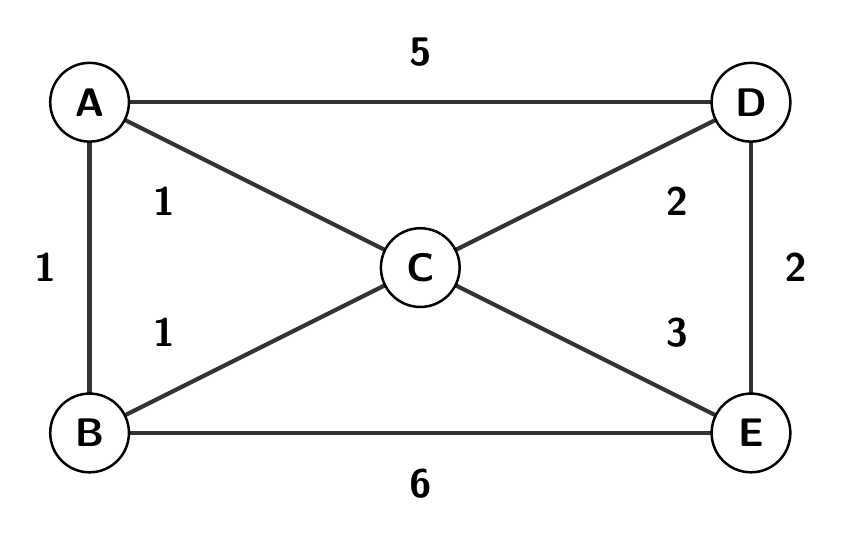
\begin{tikzpicture}[x=1mm,y=1mm]
\draw[line width=1.5pt, black!80] (7.86,51.46) -- (7.86,9.46);
\draw[line width=1.5pt, black!80] (7.86,51.46) -- (49.86,30.46);
\draw[line width=1.5pt, black!80] (7.86,9.46) -- (49.86,30.46);
\draw[line width=1.5pt, black!80] (49.86,30.46) -- (91.86,51.46);
\draw[line width=1.5pt, black!80] (49.86,30.46) -- (91.86,9.46);
\draw[line width=1.5pt, black!80] (91.86,51.46) -- (91.86,9.46);
\draw[line width=1.5pt, black!80] (7.86,51.46) -- (91.86,51.46);
\draw[line width=1.5pt, black!80] (7.86,9.46) -- (91.86,9.46);
\node[fill=white, inner sep=0, minimum width=4.40mm, minimum height=6.00mm, font=\Large\bfseries] at (2.20,30.46) {1};
\node[fill=white, inner sep=0, minimum width=4.40mm, minimum height=6.00mm, font=\Large\bfseries] at (17.28,38.79) {1};
\node[fill=white, inner sep=0, minimum width=4.40mm, minimum height=6.00mm, font=\Large\bfseries] at (17.28,22.14) {1};
\node[fill=white, inner sep=0, minimum width=4.40mm, minimum height=6.00mm, font=\Large\bfseries] at (82.45,38.79) {2};
\node[fill=white, inner sep=0, minimum width=4.40mm, minimum height=6.00mm, font=\Large\bfseries] at (82.45,22.14) {3};
\node[fill=white, inner sep=0, minimum width=4.40mm, minimum height=6.00mm, font=\Large\bfseries] at (97.53,30.46) {2};
\node[fill=white, inner sep=0, minimum width=4.40mm, minimum height=6.00mm, font=\Large\bfseries] at (49.86,57.93) {5};
\node[fill=white, inner sep=0, minimum width=4.40mm, minimum height=6.00mm, font=\Large\bfseries] at (49.86,3.00) {6};
\node[circle, draw, line width=0.9pt, fill=white, minimum size=10.00mm, inner sep=0, font=\Large\bfseries] at (7.86,51.46) {A};
\node[circle, draw, line width=0.9pt, fill=white, minimum size=10.00mm, inner sep=0, font=\Large\bfseries] at (7.86,9.46) {B};
\node[circle, draw, line width=0.9pt, fill=white, minimum size=10.00mm, inner sep=0, font=\Large\bfseries] at (49.86,30.46) {C};
\node[circle, draw, line width=0.9pt, fill=white, minimum size=10.00mm, inner sep=0, font=\Large\bfseries] at (91.86,51.46) {D};
\node[circle, draw, line width=0.9pt, fill=white, minimum size=10.00mm, inner sep=0, font=\Large\bfseries] at (91.86,9.46) {E};
\end{tikzpicture}
\end{center}\par

\vspace{3mm}
\par\begin{center}
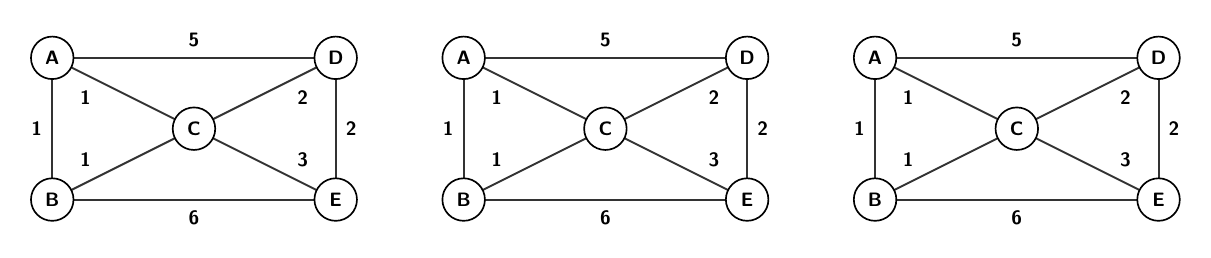
\begin{tikzpicture}[x=1mm,y=1mm]
\draw[line width=0.7pt, black!80] (3.12,21.82) -- (3.12,3.82);
\draw[line width=0.7pt, black!80] (3.12,21.82) -- (21.12,12.82);
\draw[line width=0.7pt, black!80] (3.12,3.82) -- (21.12,12.82);
\draw[line width=0.7pt, black!80] (21.12,12.82) -- (39.12,21.82);
\draw[line width=0.7pt, black!80] (21.12,12.82) -- (39.12,3.82);
\draw[line width=0.7pt, black!80] (39.12,21.82) -- (39.12,3.82);
\draw[line width=0.7pt, black!80] (3.12,21.82) -- (39.12,21.82);
\draw[line width=0.7pt, black!80] (3.12,3.82) -- (39.12,3.82);
\node[fill=white, inner sep=0, minimum width=2.30mm, minimum height=3.00mm, font=\scriptsize\bfseries] at (1.15,12.82) {1};
\node[fill=white, inner sep=0, minimum width=2.30mm, minimum height=3.00mm, font=\scriptsize\bfseries] at (7.33,16.73) {1};
\node[fill=white, inner sep=0, minimum width=2.30mm, minimum height=3.00mm, font=\scriptsize\bfseries] at (7.33,8.92) {1};
\node[fill=white, inner sep=0, minimum width=2.30mm, minimum height=3.00mm, font=\scriptsize\bfseries] at (34.92,16.73) {2};
\node[fill=white, inner sep=0, minimum width=2.30mm, minimum height=3.00mm, font=\scriptsize\bfseries] at (34.92,8.92) {3};
\node[fill=white, inner sep=0, minimum width=2.30mm, minimum height=3.00mm, font=\scriptsize\bfseries] at (41.10,12.82) {2};
\node[fill=white, inner sep=0, minimum width=2.30mm, minimum height=3.00mm, font=\scriptsize\bfseries] at (21.12,24.15) {5};
\node[fill=white, inner sep=0, minimum width=2.30mm, minimum height=3.00mm, font=\scriptsize\bfseries] at (21.12,1.50) {6};
\node[circle, draw, line width=0.6pt, fill=white, minimum size=5.40mm, inner sep=0, font=\scriptsize\bfseries] at (3.12,21.82) {A};
\node[circle, draw, line width=0.6pt, fill=white, minimum size=5.40mm, inner sep=0, font=\scriptsize\bfseries] at (3.12,3.82) {B};
\node[circle, draw, line width=0.6pt, fill=white, minimum size=5.40mm, inner sep=0, font=\scriptsize\bfseries] at (21.12,12.82) {C};
\node[circle, draw, line width=0.6pt, fill=white, minimum size=5.40mm, inner sep=0, font=\scriptsize\bfseries] at (39.12,21.82) {D};
\node[circle, draw, line width=0.6pt, fill=white, minimum size=5.40mm, inner sep=0, font=\scriptsize\bfseries] at (39.12,3.82) {E};
\draw[line width=0.7pt, black!80] (55.37,21.82) -- (55.37,3.82);
\draw[line width=0.7pt, black!80] (55.37,21.82) -- (73.37,12.82);
\draw[line width=0.7pt, black!80] (55.37,3.82) -- (73.37,12.82);
\draw[line width=0.7pt, black!80] (73.37,12.82) -- (91.37,21.82);
\draw[line width=0.7pt, black!80] (73.37,12.82) -- (91.37,3.82);
\draw[line width=0.7pt, black!80] (91.37,21.82) -- (91.37,3.82);
\draw[line width=0.7pt, black!80] (55.37,21.82) -- (91.37,21.82);
\draw[line width=0.7pt, black!80] (55.37,3.82) -- (91.37,3.82);
\node[fill=white, inner sep=0, minimum width=2.30mm, minimum height=3.00mm, font=\scriptsize\bfseries] at (53.40,12.82) {1};
\node[fill=white, inner sep=0, minimum width=2.30mm, minimum height=3.00mm, font=\scriptsize\bfseries] at (59.57,16.73) {1};
\node[fill=white, inner sep=0, minimum width=2.30mm, minimum height=3.00mm, font=\scriptsize\bfseries] at (59.57,8.92) {1};
\node[fill=white, inner sep=0, minimum width=2.30mm, minimum height=3.00mm, font=\scriptsize\bfseries] at (87.17,16.73) {2};
\node[fill=white, inner sep=0, minimum width=2.30mm, minimum height=3.00mm, font=\scriptsize\bfseries] at (87.17,8.92) {3};
\node[fill=white, inner sep=0, minimum width=2.30mm, minimum height=3.00mm, font=\scriptsize\bfseries] at (93.34,12.82) {2};
\node[fill=white, inner sep=0, minimum width=2.30mm, minimum height=3.00mm, font=\scriptsize\bfseries] at (73.37,24.15) {5};
\node[fill=white, inner sep=0, minimum width=2.30mm, minimum height=3.00mm, font=\scriptsize\bfseries] at (73.37,1.50) {6};
\node[circle, draw, line width=0.6pt, fill=white, minimum size=5.40mm, inner sep=0, font=\scriptsize\bfseries] at (55.37,21.82) {A};
\node[circle, draw, line width=0.6pt, fill=white, minimum size=5.40mm, inner sep=0, font=\scriptsize\bfseries] at (55.37,3.82) {B};
\node[circle, draw, line width=0.6pt, fill=white, minimum size=5.40mm, inner sep=0, font=\scriptsize\bfseries] at (73.37,12.82) {C};
\node[circle, draw, line width=0.6pt, fill=white, minimum size=5.40mm, inner sep=0, font=\scriptsize\bfseries] at (91.37,21.82) {D};
\node[circle, draw, line width=0.6pt, fill=white, minimum size=5.40mm, inner sep=0, font=\scriptsize\bfseries] at (91.37,3.82) {E};
\draw[line width=0.7pt, black!80] (107.62,21.82) -- (107.62,3.82);
\draw[line width=0.7pt, black!80] (107.62,21.82) -- (125.62,12.82);
\draw[line width=0.7pt, black!80] (107.62,3.82) -- (125.62,12.82);
\draw[line width=0.7pt, black!80] (125.62,12.82) -- (143.62,21.82);
\draw[line width=0.7pt, black!80] (125.62,12.82) -- (143.62,3.82);
\draw[line width=0.7pt, black!80] (143.62,21.82) -- (143.62,3.82);
\draw[line width=0.7pt, black!80] (107.62,21.82) -- (143.62,21.82);
\draw[line width=0.7pt, black!80] (107.62,3.82) -- (143.62,3.82);
\node[fill=white, inner sep=0, minimum width=2.30mm, minimum height=3.00mm, font=\scriptsize\bfseries] at (105.64,12.82) {1};
\node[fill=white, inner sep=0, minimum width=2.30mm, minimum height=3.00mm, font=\scriptsize\bfseries] at (111.82,16.73) {1};
\node[fill=white, inner sep=0, minimum width=2.30mm, minimum height=3.00mm, font=\scriptsize\bfseries] at (111.82,8.92) {1};
\node[fill=white, inner sep=0, minimum width=2.30mm, minimum height=3.00mm, font=\scriptsize\bfseries] at (139.42,16.73) {2};
\node[fill=white, inner sep=0, minimum width=2.30mm, minimum height=3.00mm, font=\scriptsize\bfseries] at (139.42,8.92) {3};
\node[fill=white, inner sep=0, minimum width=2.30mm, minimum height=3.00mm, font=\scriptsize\bfseries] at (145.59,12.82) {2};
\node[fill=white, inner sep=0, minimum width=2.30mm, minimum height=3.00mm, font=\scriptsize\bfseries] at (125.62,24.15) {5};
\node[fill=white, inner sep=0, minimum width=2.30mm, minimum height=3.00mm, font=\scriptsize\bfseries] at (125.62,1.50) {6};
\node[circle, draw, line width=0.6pt, fill=white, minimum size=5.40mm, inner sep=0, font=\scriptsize\bfseries] at (107.62,21.82) {A};
\node[circle, draw, line width=0.6pt, fill=white, minimum size=5.40mm, inner sep=0, font=\scriptsize\bfseries] at (107.62,3.82) {B};
\node[circle, draw, line width=0.6pt, fill=white, minimum size=5.40mm, inner sep=0, font=\scriptsize\bfseries] at (125.62,12.82) {C};
\node[circle, draw, line width=0.6pt, fill=white, minimum size=5.40mm, inner sep=0, font=\scriptsize\bfseries] at (143.62,21.82) {D};
\node[circle, draw, line width=0.6pt, fill=white, minimum size=5.40mm, inner sep=0, font=\scriptsize\bfseries] at (143.62,3.82) {E};
\end{tikzpicture}
\end{center}\par

\vspace{1mm}
\par\begin{center}
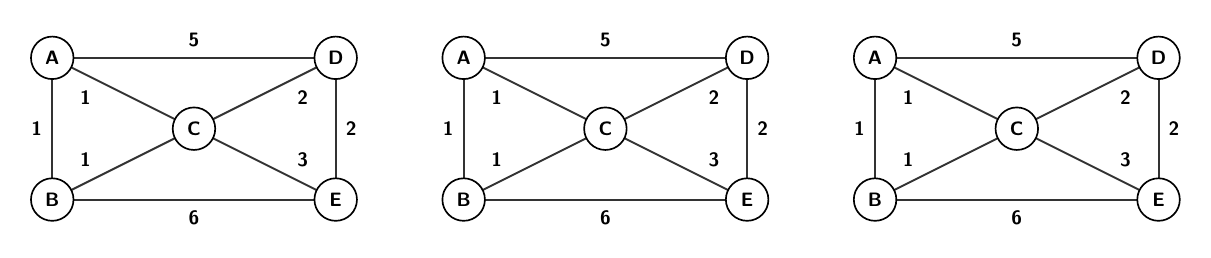
\begin{tikzpicture}[x=1mm,y=1mm]
\draw[line width=0.7pt, black!80] (3.12,21.82) -- (3.12,3.82);
\draw[line width=0.7pt, black!80] (3.12,21.82) -- (21.12,12.82);
\draw[line width=0.7pt, black!80] (3.12,3.82) -- (21.12,12.82);
\draw[line width=0.7pt, black!80] (21.12,12.82) -- (39.12,21.82);
\draw[line width=0.7pt, black!80] (21.12,12.82) -- (39.12,3.82);
\draw[line width=0.7pt, black!80] (39.12,21.82) -- (39.12,3.82);
\draw[line width=0.7pt, black!80] (3.12,21.82) -- (39.12,21.82);
\draw[line width=0.7pt, black!80] (3.12,3.82) -- (39.12,3.82);
\node[fill=white, inner sep=0, minimum width=2.30mm, minimum height=3.00mm, font=\scriptsize\bfseries] at (1.15,12.82) {1};
\node[fill=white, inner sep=0, minimum width=2.30mm, minimum height=3.00mm, font=\scriptsize\bfseries] at (7.33,16.73) {1};
\node[fill=white, inner sep=0, minimum width=2.30mm, minimum height=3.00mm, font=\scriptsize\bfseries] at (7.33,8.92) {1};
\node[fill=white, inner sep=0, minimum width=2.30mm, minimum height=3.00mm, font=\scriptsize\bfseries] at (34.92,16.73) {2};
\node[fill=white, inner sep=0, minimum width=2.30mm, minimum height=3.00mm, font=\scriptsize\bfseries] at (34.92,8.92) {3};
\node[fill=white, inner sep=0, minimum width=2.30mm, minimum height=3.00mm, font=\scriptsize\bfseries] at (41.10,12.82) {2};
\node[fill=white, inner sep=0, minimum width=2.30mm, minimum height=3.00mm, font=\scriptsize\bfseries] at (21.12,24.15) {5};
\node[fill=white, inner sep=0, minimum width=2.30mm, minimum height=3.00mm, font=\scriptsize\bfseries] at (21.12,1.50) {6};
\node[circle, draw, line width=0.6pt, fill=white, minimum size=5.40mm, inner sep=0, font=\scriptsize\bfseries] at (3.12,21.82) {A};
\node[circle, draw, line width=0.6pt, fill=white, minimum size=5.40mm, inner sep=0, font=\scriptsize\bfseries] at (3.12,3.82) {B};
\node[circle, draw, line width=0.6pt, fill=white, minimum size=5.40mm, inner sep=0, font=\scriptsize\bfseries] at (21.12,12.82) {C};
\node[circle, draw, line width=0.6pt, fill=white, minimum size=5.40mm, inner sep=0, font=\scriptsize\bfseries] at (39.12,21.82) {D};
\node[circle, draw, line width=0.6pt, fill=white, minimum size=5.40mm, inner sep=0, font=\scriptsize\bfseries] at (39.12,3.82) {E};
\draw[line width=0.7pt, black!80] (55.37,21.82) -- (55.37,3.82);
\draw[line width=0.7pt, black!80] (55.37,21.82) -- (73.37,12.82);
\draw[line width=0.7pt, black!80] (55.37,3.82) -- (73.37,12.82);
\draw[line width=0.7pt, black!80] (73.37,12.82) -- (91.37,21.82);
\draw[line width=0.7pt, black!80] (73.37,12.82) -- (91.37,3.82);
\draw[line width=0.7pt, black!80] (91.37,21.82) -- (91.37,3.82);
\draw[line width=0.7pt, black!80] (55.37,21.82) -- (91.37,21.82);
\draw[line width=0.7pt, black!80] (55.37,3.82) -- (91.37,3.82);
\node[fill=white, inner sep=0, minimum width=2.30mm, minimum height=3.00mm, font=\scriptsize\bfseries] at (53.40,12.82) {1};
\node[fill=white, inner sep=0, minimum width=2.30mm, minimum height=3.00mm, font=\scriptsize\bfseries] at (59.57,16.73) {1};
\node[fill=white, inner sep=0, minimum width=2.30mm, minimum height=3.00mm, font=\scriptsize\bfseries] at (59.57,8.92) {1};
\node[fill=white, inner sep=0, minimum width=2.30mm, minimum height=3.00mm, font=\scriptsize\bfseries] at (87.17,16.73) {2};
\node[fill=white, inner sep=0, minimum width=2.30mm, minimum height=3.00mm, font=\scriptsize\bfseries] at (87.17,8.92) {3};
\node[fill=white, inner sep=0, minimum width=2.30mm, minimum height=3.00mm, font=\scriptsize\bfseries] at (93.34,12.82) {2};
\node[fill=white, inner sep=0, minimum width=2.30mm, minimum height=3.00mm, font=\scriptsize\bfseries] at (73.37,24.15) {5};
\node[fill=white, inner sep=0, minimum width=2.30mm, minimum height=3.00mm, font=\scriptsize\bfseries] at (73.37,1.50) {6};
\node[circle, draw, line width=0.6pt, fill=white, minimum size=5.40mm, inner sep=0, font=\scriptsize\bfseries] at (55.37,21.82) {A};
\node[circle, draw, line width=0.6pt, fill=white, minimum size=5.40mm, inner sep=0, font=\scriptsize\bfseries] at (55.37,3.82) {B};
\node[circle, draw, line width=0.6pt, fill=white, minimum size=5.40mm, inner sep=0, font=\scriptsize\bfseries] at (73.37,12.82) {C};
\node[circle, draw, line width=0.6pt, fill=white, minimum size=5.40mm, inner sep=0, font=\scriptsize\bfseries] at (91.37,21.82) {D};
\node[circle, draw, line width=0.6pt, fill=white, minimum size=5.40mm, inner sep=0, font=\scriptsize\bfseries] at (91.37,3.82) {E};
\draw[line width=0.7pt, black!80] (107.62,21.82) -- (107.62,3.82);
\draw[line width=0.7pt, black!80] (107.62,21.82) -- (125.62,12.82);
\draw[line width=0.7pt, black!80] (107.62,3.82) -- (125.62,12.82);
\draw[line width=0.7pt, black!80] (125.62,12.82) -- (143.62,21.82);
\draw[line width=0.7pt, black!80] (125.62,12.82) -- (143.62,3.82);
\draw[line width=0.7pt, black!80] (143.62,21.82) -- (143.62,3.82);
\draw[line width=0.7pt, black!80] (107.62,21.82) -- (143.62,21.82);
\draw[line width=0.7pt, black!80] (107.62,3.82) -- (143.62,3.82);
\node[fill=white, inner sep=0, minimum width=2.30mm, minimum height=3.00mm, font=\scriptsize\bfseries] at (105.64,12.82) {1};
\node[fill=white, inner sep=0, minimum width=2.30mm, minimum height=3.00mm, font=\scriptsize\bfseries] at (111.82,16.73) {1};
\node[fill=white, inner sep=0, minimum width=2.30mm, minimum height=3.00mm, font=\scriptsize\bfseries] at (111.82,8.92) {1};
\node[fill=white, inner sep=0, minimum width=2.30mm, minimum height=3.00mm, font=\scriptsize\bfseries] at (139.42,16.73) {2};
\node[fill=white, inner sep=0, minimum width=2.30mm, minimum height=3.00mm, font=\scriptsize\bfseries] at (139.42,8.92) {3};
\node[fill=white, inner sep=0, minimum width=2.30mm, minimum height=3.00mm, font=\scriptsize\bfseries] at (145.59,12.82) {2};
\node[fill=white, inner sep=0, minimum width=2.30mm, minimum height=3.00mm, font=\scriptsize\bfseries] at (125.62,24.15) {5};
\node[fill=white, inner sep=0, minimum width=2.30mm, minimum height=3.00mm, font=\scriptsize\bfseries] at (125.62,1.50) {6};
\node[circle, draw, line width=0.6pt, fill=white, minimum size=5.40mm, inner sep=0, font=\scriptsize\bfseries] at (107.62,21.82) {A};
\node[circle, draw, line width=0.6pt, fill=white, minimum size=5.40mm, inner sep=0, font=\scriptsize\bfseries] at (107.62,3.82) {B};
\node[circle, draw, line width=0.6pt, fill=white, minimum size=5.40mm, inner sep=0, font=\scriptsize\bfseries] at (125.62,12.82) {C};
\node[circle, draw, line width=0.6pt, fill=white, minimum size=5.40mm, inner sep=0, font=\scriptsize\bfseries] at (143.62,21.82) {D};
\node[circle, draw, line width=0.6pt, fill=white, minimum size=5.40mm, inner sep=0, font=\scriptsize\bfseries] at (143.62,3.82) {E};
\end{tikzpicture}
\end{center}\par

\vspace{1mm}
\newpage

\prob{5} A loop is a way for the pawn to walk on markers from a place back to itself without using any marker twice. Sam says that a network with no loop whose most expensive link is as cheap as possible must be a cheapest network. Is Sam right about this map?

\par\begin{center}
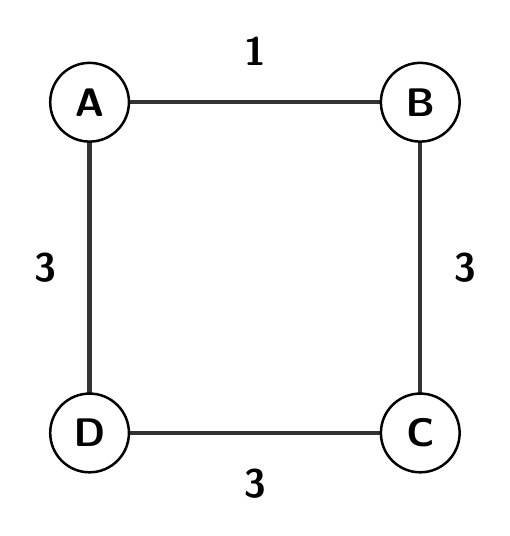
\begin{tikzpicture}[x=1mm,y=1mm]
\draw[line width=1.5pt, black!80] (7.86,51.46) -- (49.86,51.46);
\draw[line width=1.5pt, black!80] (49.86,51.46) -- (49.86,9.46);
\draw[line width=1.5pt, black!80] (49.86,9.46) -- (7.86,9.46);
\draw[line width=1.5pt, black!80] (7.86,9.46) -- (7.86,51.46);
\node[fill=white, inner sep=0, minimum width=4.40mm, minimum height=6.00mm, font=\Large\bfseries] at (28.86,57.93) {1};
\node[fill=white, inner sep=0, minimum width=4.40mm, minimum height=6.00mm, font=\Large\bfseries] at (55.53,30.46) {3};
\node[fill=white, inner sep=0, minimum width=4.40mm, minimum height=6.00mm, font=\Large\bfseries] at (28.86,3.00) {3};
\node[fill=white, inner sep=0, minimum width=4.40mm, minimum height=6.00mm, font=\Large\bfseries] at (2.20,30.46) {3};
\node[circle, draw, line width=0.9pt, fill=white, minimum size=10.00mm, inner sep=0, font=\Large\bfseries] at (7.86,51.46) {A};
\node[circle, draw, line width=0.9pt, fill=white, minimum size=10.00mm, inner sep=0, font=\Large\bfseries] at (49.86,51.46) {B};
\node[circle, draw, line width=0.9pt, fill=white, minimum size=10.00mm, inner sep=0, font=\Large\bfseries] at (49.86,9.46) {C};
\node[circle, draw, line width=0.9pt, fill=white, minimum size=10.00mm, inner sep=0, font=\Large\bfseries] at (7.86,9.46) {D};
\end{tikzpicture}
\end{center}\par

\vspace{28mm}
\prob{6} On a map with no squares, is the route between two places along a cheapest network always a route whose most expensive link is as cheap as possible? Can two cheapest networks of such a map have different lists of prices? Can you tell the cost of a cheapest network from the groups, without choosing a network? Explain.
\newpage

\prob{7} On a trip, the pawn walks from one place to another along any links, and you pay each link's price every time the pawn walks along it. Write the trip by its letters, and pay when the trip is over.

\par\begin{center}
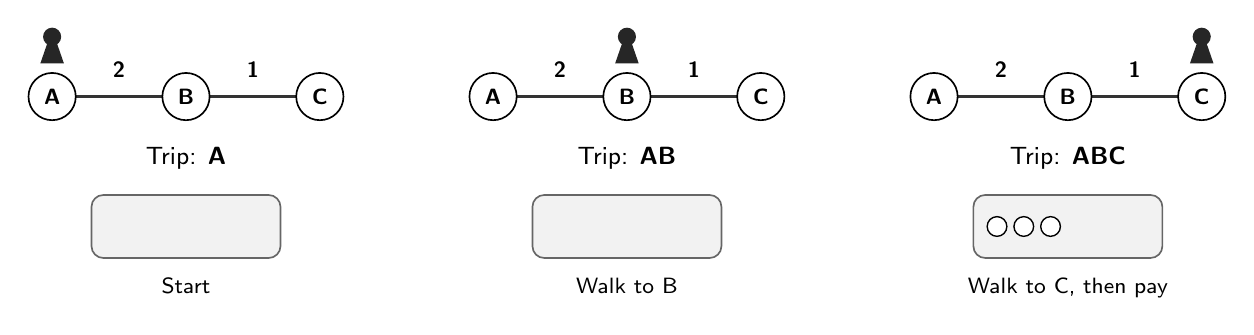
\begin{tikzpicture}[x=1mm,y=1mm]
\draw[line width=0.8pt, black!80] (3.00,25.00) -- (20.00,25.00);
\draw[line width=0.8pt, black!80] (20.00,25.00) -- (37.00,25.00);
\node[fill=white, inner sep=0, minimum width=2.80mm, minimum height=3.40mm, font=\footnotesize\bfseries] at (11.50,28.44) {2};
\node[fill=white, inner sep=0, minimum width=2.80mm, minimum height=3.40mm, font=\footnotesize\bfseries] at (28.50,28.44) {1};
\node[circle, draw, line width=0.6pt, fill=white, minimum size=6.00mm, inner sep=0, font=\footnotesize\bfseries] at (3.00,25.00) {A};
\node[circle, draw, line width=0.6pt, fill=white, minimum size=6.00mm, inner sep=0, font=\footnotesize\bfseries] at (20.00,25.00) {B};
\node[circle, draw, line width=0.6pt, fill=white, minimum size=6.00mm, inner sep=0, font=\footnotesize\bfseries] at (37.00,25.00) {C};
\fill[black!85] (1.50,29.20) -- (4.50,29.20) -- (3.60,31.80) -- (2.40,31.80) -- cycle;\fill[black!85] (3.00,32.60) circle (1.15mm);
\node[font=\small, anchor=south] at (20.00,14.5) {Trip: \textbf{A}};
\draw[black!60, line width=0.6pt, fill=black!5, rounded corners=1.5mm] (8.00,4.50) rectangle (32.00,12.50);
\node[font=\footnotesize, anchor=north, align=center] at (20.00,3.20) {Start};
\draw[line width=0.8pt, black!80] (59.00,25.00) -- (76.00,25.00);
\draw[line width=0.8pt, black!80] (76.00,25.00) -- (93.00,25.00);
\node[fill=white, inner sep=0, minimum width=2.80mm, minimum height=3.40mm, font=\footnotesize\bfseries] at (67.50,28.44) {2};
\node[fill=white, inner sep=0, minimum width=2.80mm, minimum height=3.40mm, font=\footnotesize\bfseries] at (84.50,28.44) {1};
\node[circle, draw, line width=0.6pt, fill=white, minimum size=6.00mm, inner sep=0, font=\footnotesize\bfseries] at (59.00,25.00) {A};
\node[circle, draw, line width=0.6pt, fill=white, minimum size=6.00mm, inner sep=0, font=\footnotesize\bfseries] at (76.00,25.00) {B};
\node[circle, draw, line width=0.6pt, fill=white, minimum size=6.00mm, inner sep=0, font=\footnotesize\bfseries] at (93.00,25.00) {C};
\fill[black!85] (74.50,29.20) -- (77.50,29.20) -- (76.60,31.80) -- (75.40,31.80) -- cycle;\fill[black!85] (76.00,32.60) circle (1.15mm);
\node[font=\small, anchor=south] at (76.00,14.5) {Trip: \textbf{AB}};
\draw[black!60, line width=0.6pt, fill=black!5, rounded corners=1.5mm] (64.00,4.50) rectangle (88.00,12.50);
\node[font=\footnotesize, anchor=north, align=center] at (76.00,3.20) {Walk to B};
\draw[line width=0.8pt, black!80] (115.00,25.00) -- (132.00,25.00);
\draw[line width=0.8pt, black!80] (132.00,25.00) -- (149.00,25.00);
\node[fill=white, inner sep=0, minimum width=2.80mm, minimum height=3.40mm, font=\footnotesize\bfseries] at (123.50,28.44) {2};
\node[fill=white, inner sep=0, minimum width=2.80mm, minimum height=3.40mm, font=\footnotesize\bfseries] at (140.50,28.44) {1};
\node[circle, draw, line width=0.6pt, fill=white, minimum size=6.00mm, inner sep=0, font=\footnotesize\bfseries] at (115.00,25.00) {A};
\node[circle, draw, line width=0.6pt, fill=white, minimum size=6.00mm, inner sep=0, font=\footnotesize\bfseries] at (132.00,25.00) {B};
\node[circle, draw, line width=0.6pt, fill=white, minimum size=6.00mm, inner sep=0, font=\footnotesize\bfseries] at (149.00,25.00) {C};
\fill[black!85] (147.50,29.20) -- (150.50,29.20) -- (149.60,31.80) -- (148.40,31.80) -- cycle;\fill[black!85] (149.00,32.60) circle (1.15mm);
\node[font=\small, anchor=south] at (132.00,14.5) {Trip: \textbf{ABC}};
\draw[black!60, line width=0.6pt, fill=black!5, rounded corners=1.5mm] (120.00,4.50) rectangle (144.00,12.50);
\draw[line width=0.5pt, fill=white] (123.00,8.50) circle (1.25mm);
\draw[line width=0.5pt, fill=white] (126.40,8.50) circle (1.25mm);
\draw[line width=0.5pt, fill=white] (129.80,8.50) circle (1.25mm);
\node[font=\footnotesize, anchor=north, align=center] at (132.00,3.20) {Walk to C, then pay};
\end{tikzpicture}
\end{center}\par

On each map, find a cheapest network and a cheapest trip from A to D.

\vspace{4mm}

\par\begin{center}
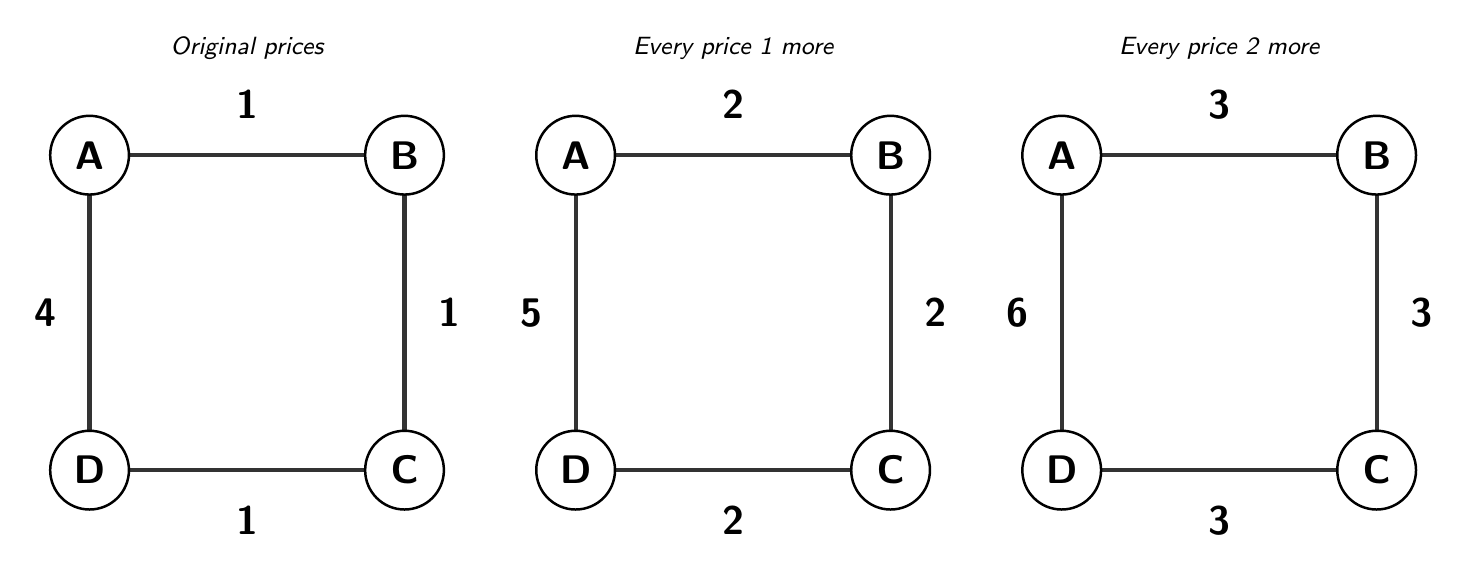
\begin{tikzpicture}[x=1mm,y=1mm]
\draw[line width=1.5pt, black!80] (7.86,49.46) -- (47.86,49.46);
\draw[line width=1.5pt, black!80] (47.86,49.46) -- (47.86,9.46);
\draw[line width=1.5pt, black!80] (47.86,9.46) -- (7.86,9.46);
\draw[line width=1.5pt, black!80] (7.86,9.46) -- (7.86,49.46);
\node[fill=white, inner sep=0, minimum width=4.40mm, minimum height=6.00mm, font=\Large\bfseries] at (27.86,55.93) {1};
\node[fill=white, inner sep=0, minimum width=4.40mm, minimum height=6.00mm, font=\Large\bfseries] at (53.53,29.46) {1};
\node[fill=white, inner sep=0, minimum width=4.40mm, minimum height=6.00mm, font=\Large\bfseries] at (27.86,3.00) {1};
\node[fill=white, inner sep=0, minimum width=4.40mm, minimum height=6.00mm, font=\Large\bfseries] at (2.20,29.46) {4};
\node[circle, draw, line width=0.9pt, fill=white, minimum size=10.00mm, inner sep=0, font=\Large\bfseries] at (7.86,49.46) {A};
\node[circle, draw, line width=0.9pt, fill=white, minimum size=10.00mm, inner sep=0, font=\Large\bfseries] at (47.86,49.46) {B};
\node[circle, draw, line width=0.9pt, fill=white, minimum size=10.00mm, inner sep=0, font=\Large\bfseries] at (47.86,9.46) {C};
\node[circle, draw, line width=0.9pt, fill=white, minimum size=10.00mm, inner sep=0, font=\Large\bfseries] at (7.86,9.46) {D};
\node[font=\small, anchor=south, align=center] at (27.86,60.43) {\itshape Original prices};
\draw[line width=1.5pt, black!80] (69.59,49.46) -- (109.59,49.46);
\draw[line width=1.5pt, black!80] (109.59,49.46) -- (109.59,9.46);
\draw[line width=1.5pt, black!80] (109.59,9.46) -- (69.59,9.46);
\draw[line width=1.5pt, black!80] (69.59,9.46) -- (69.59,49.46);
\node[fill=white, inner sep=0, minimum width=4.40mm, minimum height=6.00mm, font=\Large\bfseries] at (89.59,55.93) {2};
\node[fill=white, inner sep=0, minimum width=4.40mm, minimum height=6.00mm, font=\Large\bfseries] at (115.26,29.46) {2};
\node[fill=white, inner sep=0, minimum width=4.40mm, minimum height=6.00mm, font=\Large\bfseries] at (89.59,3.00) {2};
\node[fill=white, inner sep=0, minimum width=4.40mm, minimum height=6.00mm, font=\Large\bfseries] at (63.93,29.46) {5};
\node[circle, draw, line width=0.9pt, fill=white, minimum size=10.00mm, inner sep=0, font=\Large\bfseries] at (69.59,49.46) {A};
\node[circle, draw, line width=0.9pt, fill=white, minimum size=10.00mm, inner sep=0, font=\Large\bfseries] at (109.59,49.46) {B};
\node[circle, draw, line width=0.9pt, fill=white, minimum size=10.00mm, inner sep=0, font=\Large\bfseries] at (109.59,9.46) {C};
\node[circle, draw, line width=0.9pt, fill=white, minimum size=10.00mm, inner sep=0, font=\Large\bfseries] at (69.59,9.46) {D};
\node[font=\small, anchor=south, align=center] at (89.59,60.43) {\itshape Every price 1 more};
\draw[line width=1.5pt, black!80] (131.32,49.46) -- (171.32,49.46);
\draw[line width=1.5pt, black!80] (171.32,49.46) -- (171.32,9.46);
\draw[line width=1.5pt, black!80] (171.32,9.46) -- (131.32,9.46);
\draw[line width=1.5pt, black!80] (131.32,9.46) -- (131.32,49.46);
\node[fill=white, inner sep=0, minimum width=4.40mm, minimum height=6.00mm, font=\Large\bfseries] at (151.32,55.93) {3};
\node[fill=white, inner sep=0, minimum width=4.40mm, minimum height=6.00mm, font=\Large\bfseries] at (176.99,29.46) {3};
\node[fill=white, inner sep=0, minimum width=4.40mm, minimum height=6.00mm, font=\Large\bfseries] at (151.32,3.00) {3};
\node[fill=white, inner sep=0, minimum width=4.40mm, minimum height=6.00mm, font=\Large\bfseries] at (125.66,29.46) {6};
\node[circle, draw, line width=0.9pt, fill=white, minimum size=10.00mm, inner sep=0, font=\Large\bfseries] at (131.32,49.46) {A};
\node[circle, draw, line width=0.9pt, fill=white, minimum size=10.00mm, inner sep=0, font=\Large\bfseries] at (171.32,49.46) {B};
\node[circle, draw, line width=0.9pt, fill=white, minimum size=10.00mm, inner sep=0, font=\Large\bfseries] at (171.32,9.46) {C};
\node[circle, draw, line width=0.9pt, fill=white, minimum size=10.00mm, inner sep=0, font=\Large\bfseries] at (131.32,9.46) {D};
\node[font=\small, anchor=south, align=center] at (151.32,60.43) {\itshape Every price 2 more};
\end{tikzpicture}
\end{center}\par

\vspace{3mm}
\begin{center}
\begin{minipage}[t]{58mm}\small
Network \ans{40mm}\\[1.5mm]
costs \ans{12mm}\\[7mm]
Trip \ans{44mm}\\[1.5mm]
costs \ans{12mm}
\end{minipage}\hfill\begin{minipage}[t]{58mm}\small
Network \ans{40mm}\\[1.5mm]
costs \ans{12mm}\\[7mm]
Trip \ans{44mm}\\[1.5mm]
costs \ans{12mm}
\end{minipage}\hfill\begin{minipage}[t]{58mm}\small
Network \ans{40mm}\\[1.5mm]
costs \ans{12mm}\\[7mm]
Trip \ans{44mm}\\[1.5mm]
costs \ans{12mm}
\end{minipage}
\end{center}
\newpage

\prob{8} On each map, find a cheapest network and every cheapest trip from A to F. Which ways of changing every price can change the cheapest networks of a map with no squares? Which can change its cheapest trips? Explain.

\vspace{2mm}

\noindent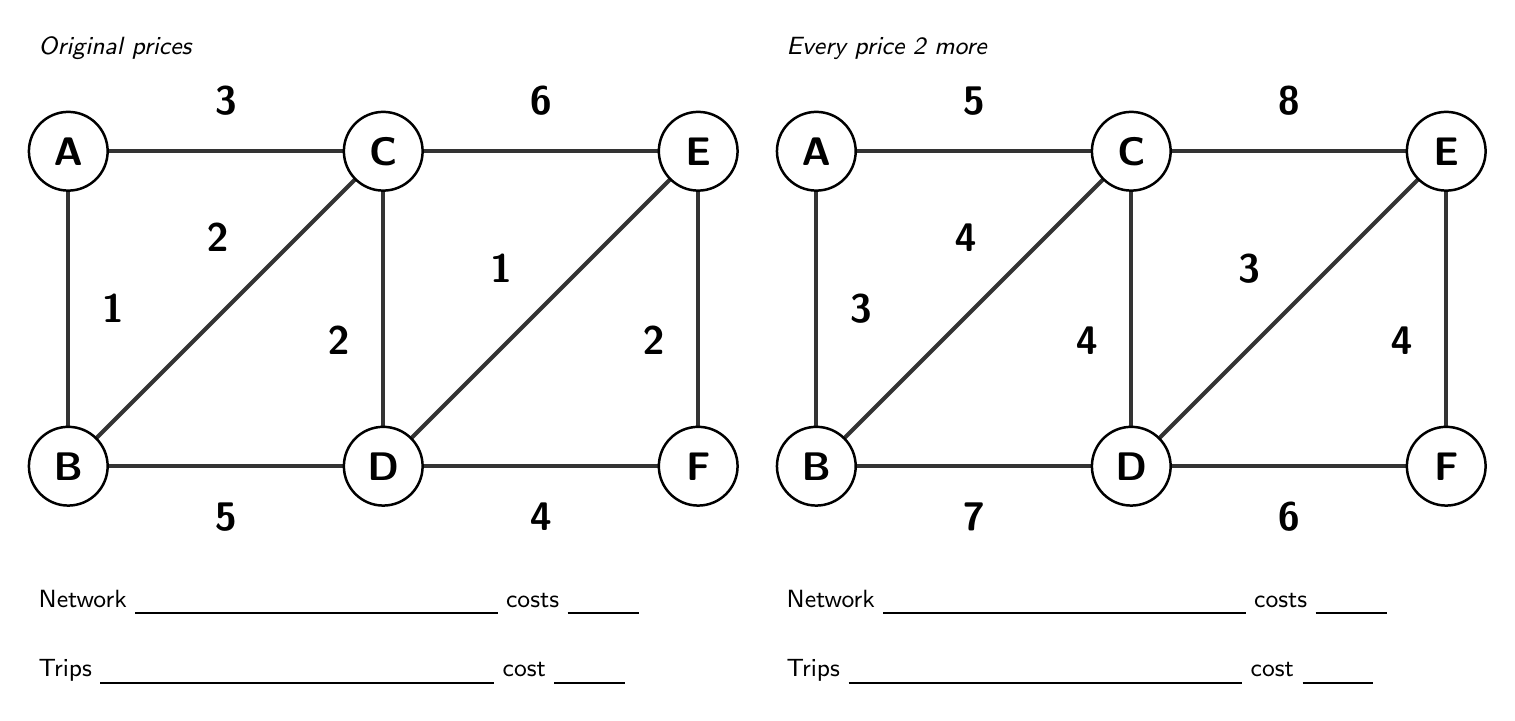
\begin{tikzpicture}[x=1mm,y=1mm]
\draw[line width=1.5pt, black!80] (5.00,71.46) -- (5.00,31.46);
\draw[line width=1.5pt, black!80] (5.00,31.46) -- (45.00,71.46);
\draw[line width=1.5pt, black!80] (5.00,71.46) -- (45.00,71.46);
\draw[line width=1.5pt, black!80] (45.00,71.46) -- (45.00,31.46);
\draw[line width=1.5pt, black!80] (45.00,31.46) -- (85.00,71.46);
\draw[line width=1.5pt, black!80] (85.00,71.46) -- (85.00,31.46);
\draw[line width=1.5pt, black!80] (45.00,31.46) -- (85.00,31.46);
\draw[line width=1.5pt, black!80] (5.00,31.46) -- (45.00,31.46);
\draw[line width=1.5pt, black!80] (45.00,71.46) -- (85.00,71.46);
\node[fill=white, inner sep=0, minimum width=4.40mm, minimum height=6.00mm, font=\Large\bfseries] at (10.66,51.46) {1};
\node[fill=white, inner sep=0, minimum width=4.40mm, minimum height=6.00mm, font=\Large\bfseries] at (23.95,60.51) {2};
\node[fill=white, inner sep=0, minimum width=4.40mm, minimum height=6.00mm, font=\Large\bfseries] at (25.00,77.93) {3};
\node[fill=white, inner sep=0, minimum width=4.40mm, minimum height=6.00mm, font=\Large\bfseries] at (39.34,47.46) {2};
\node[fill=white, inner sep=0, minimum width=4.40mm, minimum height=6.00mm, font=\Large\bfseries] at (59.95,56.51) {1};
\node[fill=white, inner sep=0, minimum width=4.40mm, minimum height=6.00mm, font=\Large\bfseries] at (79.34,47.46) {2};
\node[fill=white, inner sep=0, minimum width=4.40mm, minimum height=6.00mm, font=\Large\bfseries] at (65.00,25.00) {4};
\node[fill=white, inner sep=0, minimum width=4.40mm, minimum height=6.00mm, font=\Large\bfseries] at (25.00,25.00) {5};
\node[fill=white, inner sep=0, minimum width=4.40mm, minimum height=6.00mm, font=\Large\bfseries] at (65.00,77.93) {6};
\node[circle, draw, line width=0.9pt, fill=white, minimum size=10.00mm, inner sep=0, font=\Large\bfseries] at (5.00,71.46) {A};
\node[circle, draw, line width=0.9pt, fill=white, minimum size=10.00mm, inner sep=0, font=\Large\bfseries] at (45.00,71.46) {C};
\node[circle, draw, line width=0.9pt, fill=white, minimum size=10.00mm, inner sep=0, font=\Large\bfseries] at (85.00,71.46) {E};
\node[circle, draw, line width=0.9pt, fill=white, minimum size=10.00mm, inner sep=0, font=\Large\bfseries] at (5.00,31.46) {B};
\node[circle, draw, line width=0.9pt, fill=white, minimum size=10.00mm, inner sep=0, font=\Large\bfseries] at (45.00,31.46) {D};
\node[circle, draw, line width=0.9pt, fill=white, minimum size=10.00mm, inner sep=0, font=\Large\bfseries] at (85.00,31.46) {F};
\node[anchor=south west, font=\small\itshape] at (0.00,81.93) {Original prices};
\node[anchor=north west, font=\small, align=left] at (0.00,17) {Network \ans{46mm} costs \ans{9mm}\\[5mm] Trips \ans{50mm} cost \ans{9mm}};
\draw[line width=1.5pt, black!80] (100.00,71.46) -- (100.00,31.46);
\draw[line width=1.5pt, black!80] (100.00,31.46) -- (140.00,71.46);
\draw[line width=1.5pt, black!80] (100.00,71.46) -- (140.00,71.46);
\draw[line width=1.5pt, black!80] (140.00,71.46) -- (140.00,31.46);
\draw[line width=1.5pt, black!80] (140.00,31.46) -- (180.00,71.46);
\draw[line width=1.5pt, black!80] (180.00,71.46) -- (180.00,31.46);
\draw[line width=1.5pt, black!80] (140.00,31.46) -- (180.00,31.46);
\draw[line width=1.5pt, black!80] (100.00,31.46) -- (140.00,31.46);
\draw[line width=1.5pt, black!80] (140.00,71.46) -- (180.00,71.46);
\node[fill=white, inner sep=0, minimum width=4.40mm, minimum height=6.00mm, font=\Large\bfseries] at (105.66,51.46) {3};
\node[fill=white, inner sep=0, minimum width=4.40mm, minimum height=6.00mm, font=\Large\bfseries] at (118.95,60.51) {4};
\node[fill=white, inner sep=0, minimum width=4.40mm, minimum height=6.00mm, font=\Large\bfseries] at (120.00,77.93) {5};
\node[fill=white, inner sep=0, minimum width=4.40mm, minimum height=6.00mm, font=\Large\bfseries] at (134.34,47.46) {4};
\node[fill=white, inner sep=0, minimum width=4.40mm, minimum height=6.00mm, font=\Large\bfseries] at (154.95,56.51) {3};
\node[fill=white, inner sep=0, minimum width=4.40mm, minimum height=6.00mm, font=\Large\bfseries] at (174.34,47.46) {4};
\node[fill=white, inner sep=0, minimum width=4.40mm, minimum height=6.00mm, font=\Large\bfseries] at (160.00,25.00) {6};
\node[fill=white, inner sep=0, minimum width=4.40mm, minimum height=6.00mm, font=\Large\bfseries] at (120.00,25.00) {7};
\node[fill=white, inner sep=0, minimum width=4.40mm, minimum height=6.00mm, font=\Large\bfseries] at (160.00,77.93) {8};
\node[circle, draw, line width=0.9pt, fill=white, minimum size=10.00mm, inner sep=0, font=\Large\bfseries] at (100.00,71.46) {A};
\node[circle, draw, line width=0.9pt, fill=white, minimum size=10.00mm, inner sep=0, font=\Large\bfseries] at (140.00,71.46) {C};
\node[circle, draw, line width=0.9pt, fill=white, minimum size=10.00mm, inner sep=0, font=\Large\bfseries] at (180.00,71.46) {E};
\node[circle, draw, line width=0.9pt, fill=white, minimum size=10.00mm, inner sep=0, font=\Large\bfseries] at (100.00,31.46) {B};
\node[circle, draw, line width=0.9pt, fill=white, minimum size=10.00mm, inner sep=0, font=\Large\bfseries] at (140.00,31.46) {D};
\node[circle, draw, line width=0.9pt, fill=white, minimum size=10.00mm, inner sep=0, font=\Large\bfseries] at (180.00,31.46) {F};
\node[anchor=south west, font=\small\itshape] at (95.00,81.93) {Every price 2 more};
\node[anchor=north west, font=\small, align=left] at (95.00,17) {Network \ans{46mm} costs \ans{9mm}\\[5mm] Trips \ans{50mm} cost \ans{9mm}};
\end{tikzpicture}\par\vspace{2mm}

\noindent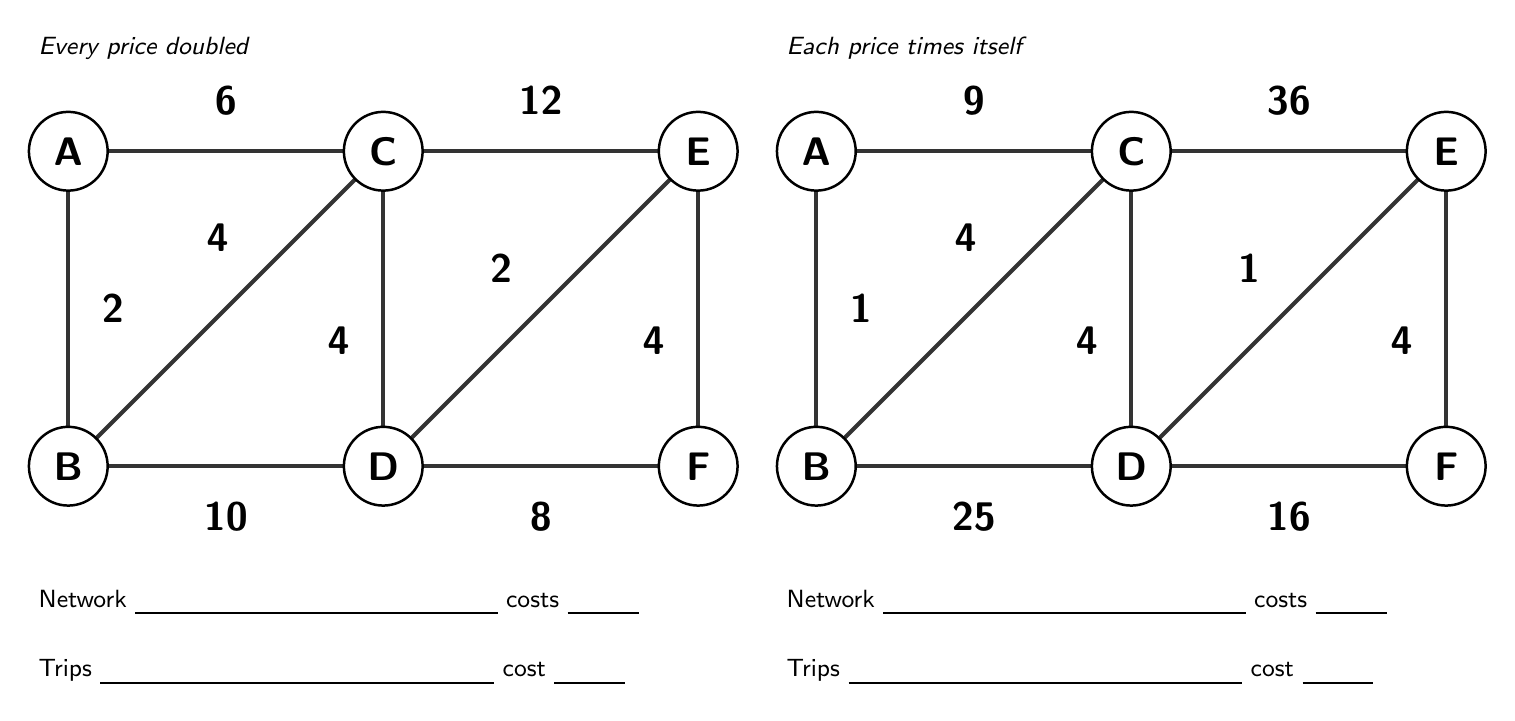
\begin{tikzpicture}[x=1mm,y=1mm]
\draw[line width=1.5pt, black!80] (5.00,71.46) -- (5.00,31.46);
\draw[line width=1.5pt, black!80] (5.00,31.46) -- (45.00,71.46);
\draw[line width=1.5pt, black!80] (5.00,71.46) -- (45.00,71.46);
\draw[line width=1.5pt, black!80] (45.00,71.46) -- (45.00,31.46);
\draw[line width=1.5pt, black!80] (45.00,31.46) -- (85.00,71.46);
\draw[line width=1.5pt, black!80] (85.00,71.46) -- (85.00,31.46);
\draw[line width=1.5pt, black!80] (45.00,31.46) -- (85.00,31.46);
\draw[line width=1.5pt, black!80] (5.00,31.46) -- (45.00,31.46);
\draw[line width=1.5pt, black!80] (45.00,71.46) -- (85.00,71.46);
\node[fill=white, inner sep=0, minimum width=4.40mm, minimum height=6.00mm, font=\Large\bfseries] at (10.66,51.46) {2};
\node[fill=white, inner sep=0, minimum width=4.40mm, minimum height=6.00mm, font=\Large\bfseries] at (23.95,60.51) {4};
\node[fill=white, inner sep=0, minimum width=4.40mm, minimum height=6.00mm, font=\Large\bfseries] at (25.00,77.93) {6};
\node[fill=white, inner sep=0, minimum width=4.40mm, minimum height=6.00mm, font=\Large\bfseries] at (39.34,47.46) {4};
\node[fill=white, inner sep=0, minimum width=4.40mm, minimum height=6.00mm, font=\Large\bfseries] at (59.95,56.51) {2};
\node[fill=white, inner sep=0, minimum width=4.40mm, minimum height=6.00mm, font=\Large\bfseries] at (79.34,47.46) {4};
\node[fill=white, inner sep=0, minimum width=4.40mm, minimum height=6.00mm, font=\Large\bfseries] at (65.00,25.00) {8};
\node[fill=white, inner sep=0, minimum width=7.60mm, minimum height=6.00mm, font=\Large\bfseries] at (25.00,25.00) {10};
\node[fill=white, inner sep=0, minimum width=7.60mm, minimum height=6.00mm, font=\Large\bfseries] at (65.00,77.93) {12};
\node[circle, draw, line width=0.9pt, fill=white, minimum size=10.00mm, inner sep=0, font=\Large\bfseries] at (5.00,71.46) {A};
\node[circle, draw, line width=0.9pt, fill=white, minimum size=10.00mm, inner sep=0, font=\Large\bfseries] at (45.00,71.46) {C};
\node[circle, draw, line width=0.9pt, fill=white, minimum size=10.00mm, inner sep=0, font=\Large\bfseries] at (85.00,71.46) {E};
\node[circle, draw, line width=0.9pt, fill=white, minimum size=10.00mm, inner sep=0, font=\Large\bfseries] at (5.00,31.46) {B};
\node[circle, draw, line width=0.9pt, fill=white, minimum size=10.00mm, inner sep=0, font=\Large\bfseries] at (45.00,31.46) {D};
\node[circle, draw, line width=0.9pt, fill=white, minimum size=10.00mm, inner sep=0, font=\Large\bfseries] at (85.00,31.46) {F};
\node[anchor=south west, font=\small\itshape] at (0.00,81.93) {Every price doubled};
\node[anchor=north west, font=\small, align=left] at (0.00,17) {Network \ans{46mm} costs \ans{9mm}\\[5mm] Trips \ans{50mm} cost \ans{9mm}};
\draw[line width=1.5pt, black!80] (100.00,71.46) -- (100.00,31.46);
\draw[line width=1.5pt, black!80] (100.00,31.46) -- (140.00,71.46);
\draw[line width=1.5pt, black!80] (100.00,71.46) -- (140.00,71.46);
\draw[line width=1.5pt, black!80] (140.00,71.46) -- (140.00,31.46);
\draw[line width=1.5pt, black!80] (140.00,31.46) -- (180.00,71.46);
\draw[line width=1.5pt, black!80] (180.00,71.46) -- (180.00,31.46);
\draw[line width=1.5pt, black!80] (140.00,31.46) -- (180.00,31.46);
\draw[line width=1.5pt, black!80] (100.00,31.46) -- (140.00,31.46);
\draw[line width=1.5pt, black!80] (140.00,71.46) -- (180.00,71.46);
\node[fill=white, inner sep=0, minimum width=4.40mm, minimum height=6.00mm, font=\Large\bfseries] at (105.66,51.46) {1};
\node[fill=white, inner sep=0, minimum width=4.40mm, minimum height=6.00mm, font=\Large\bfseries] at (118.95,60.51) {4};
\node[fill=white, inner sep=0, minimum width=4.40mm, minimum height=6.00mm, font=\Large\bfseries] at (120.00,77.93) {9};
\node[fill=white, inner sep=0, minimum width=4.40mm, minimum height=6.00mm, font=\Large\bfseries] at (134.34,47.46) {4};
\node[fill=white, inner sep=0, minimum width=4.40mm, minimum height=6.00mm, font=\Large\bfseries] at (154.95,56.51) {1};
\node[fill=white, inner sep=0, minimum width=4.40mm, minimum height=6.00mm, font=\Large\bfseries] at (174.34,47.46) {4};
\node[fill=white, inner sep=0, minimum width=7.60mm, minimum height=6.00mm, font=\Large\bfseries] at (160.00,25.00) {16};
\node[fill=white, inner sep=0, minimum width=7.60mm, minimum height=6.00mm, font=\Large\bfseries] at (120.00,25.00) {25};
\node[fill=white, inner sep=0, minimum width=7.60mm, minimum height=6.00mm, font=\Large\bfseries] at (160.00,77.93) {36};
\node[circle, draw, line width=0.9pt, fill=white, minimum size=10.00mm, inner sep=0, font=\Large\bfseries] at (100.00,71.46) {A};
\node[circle, draw, line width=0.9pt, fill=white, minimum size=10.00mm, inner sep=0, font=\Large\bfseries] at (140.00,71.46) {C};
\node[circle, draw, line width=0.9pt, fill=white, minimum size=10.00mm, inner sep=0, font=\Large\bfseries] at (180.00,71.46) {E};
\node[circle, draw, line width=0.9pt, fill=white, minimum size=10.00mm, inner sep=0, font=\Large\bfseries] at (100.00,31.46) {B};
\node[circle, draw, line width=0.9pt, fill=white, minimum size=10.00mm, inner sep=0, font=\Large\bfseries] at (140.00,31.46) {D};
\node[circle, draw, line width=0.9pt, fill=white, minimum size=10.00mm, inner sep=0, font=\Large\bfseries] at (180.00,31.46) {F};
\node[anchor=south west, font=\small\itshape] at (95.00,81.93) {Each price times itself};
\node[anchor=north west, font=\small, align=left] at (95.00,17) {Network \ans{46mm} costs \ans{9mm}\\[5mm] Trips \ans{50mm} cost \ans{9mm}};
\end{tikzpicture}\par\vspace{2mm}

\newpage

\prob{9} On each map, find every cheapest network.

\par\begin{center}
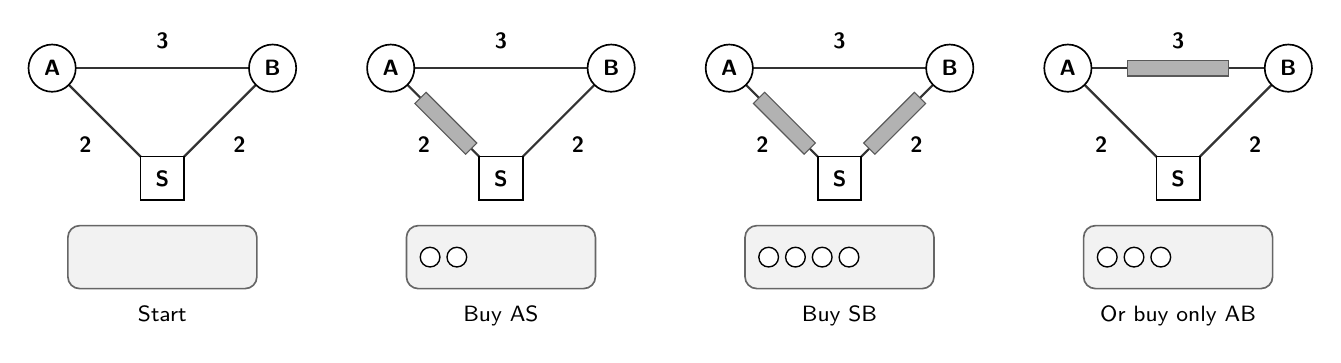
\begin{tikzpicture}[x=1mm,y=1mm]
\draw[line width=0.8pt, black!80] (3.00,29.00) -- (31.00,29.00);
\draw[line width=0.8pt, black!80] (3.00,29.00) -- (17.00,15.00);
\draw[line width=0.8pt, black!80] (17.00,15.00) -- (31.00,29.00);
\node[fill=white, inner sep=0, minimum width=2.80mm, minimum height=3.40mm, font=\footnotesize\bfseries] at (17.00,32.44) {3};
\node[fill=white, inner sep=0, minimum width=2.80mm, minimum height=3.40mm, font=\footnotesize\bfseries] at (7.22,19.22) {2};
\node[fill=white, inner sep=0, minimum width=2.80mm, minimum height=3.40mm, font=\footnotesize\bfseries] at (26.78,19.22) {2};
\node[circle, draw, line width=0.6pt, fill=white, minimum size=6.00mm, inner sep=0, font=\footnotesize\bfseries] at (3.00,29.00) {A};
\node[circle, draw, line width=0.6pt, fill=white, minimum size=6.00mm, inner sep=0, font=\footnotesize\bfseries] at (31.00,29.00) {B};
\node[rectangle, draw, line width=0.6pt, fill=white, minimum size=5.52mm, inner sep=0, font=\footnotesize\bfseries] at (17.00,15.00) {S};
\draw[black!60, line width=0.6pt, fill=black!5, rounded corners=1.5mm] (5.00,1.00) rectangle (29.00,9.00);
\node[font=\footnotesize, anchor=north, align=center] at (17.00,0.00) {Start};
\draw[line width=0.8pt, black!80] (46.00,29.00) -- (74.00,29.00);
\draw[line width=0.8pt, black!80] (46.00,29.00) -- (60.00,15.00);
\draw[line width=0.8pt, black!80] (60.00,15.00) -- (74.00,29.00);
\filldraw[fill=black!30, draw=black!65, line width=0.4pt] (50.49,25.93) -- (56.93,19.49) -- (55.51,18.07) -- (49.07,24.51) -- cycle;
\node[fill=white, inner sep=0, minimum width=2.80mm, minimum height=3.40mm, font=\footnotesize\bfseries] at (60.00,32.44) {3};
\node[fill=white, inner sep=0, minimum width=2.80mm, minimum height=3.40mm, font=\footnotesize\bfseries] at (50.22,19.22) {2};
\node[fill=white, inner sep=0, minimum width=2.80mm, minimum height=3.40mm, font=\footnotesize\bfseries] at (69.78,19.22) {2};
\node[circle, draw, line width=0.6pt, fill=white, minimum size=6.00mm, inner sep=0, font=\footnotesize\bfseries] at (46.00,29.00) {A};
\node[circle, draw, line width=0.6pt, fill=white, minimum size=6.00mm, inner sep=0, font=\footnotesize\bfseries] at (74.00,29.00) {B};
\node[rectangle, draw, line width=0.6pt, fill=white, minimum size=5.52mm, inner sep=0, font=\footnotesize\bfseries] at (60.00,15.00) {S};
\draw[black!60, line width=0.6pt, fill=black!5, rounded corners=1.5mm] (48.00,1.00) rectangle (72.00,9.00);
\draw[line width=0.5pt, fill=white] (51.00,5.00) circle (1.25mm);
\draw[line width=0.5pt, fill=white] (54.40,5.00) circle (1.25mm);
\node[font=\footnotesize, anchor=north, align=center] at (60.00,0.00) {Buy AS};
\draw[line width=0.8pt, black!80] (89.00,29.00) -- (117.00,29.00);
\draw[line width=0.8pt, black!80] (89.00,29.00) -- (103.00,15.00);
\draw[line width=0.8pt, black!80] (103.00,15.00) -- (117.00,29.00);
\filldraw[fill=black!30, draw=black!65, line width=0.4pt] (93.49,25.93) -- (99.93,19.49) -- (98.51,18.07) -- (92.07,24.51) -- cycle;
\filldraw[fill=black!30, draw=black!65, line width=0.4pt] (106.07,19.49) -- (112.51,25.93) -- (113.93,24.51) -- (107.49,18.07) -- cycle;
\node[fill=white, inner sep=0, minimum width=2.80mm, minimum height=3.40mm, font=\footnotesize\bfseries] at (103.00,32.44) {3};
\node[fill=white, inner sep=0, minimum width=2.80mm, minimum height=3.40mm, font=\footnotesize\bfseries] at (93.22,19.22) {2};
\node[fill=white, inner sep=0, minimum width=2.80mm, minimum height=3.40mm, font=\footnotesize\bfseries] at (112.78,19.22) {2};
\node[circle, draw, line width=0.6pt, fill=white, minimum size=6.00mm, inner sep=0, font=\footnotesize\bfseries] at (89.00,29.00) {A};
\node[circle, draw, line width=0.6pt, fill=white, minimum size=6.00mm, inner sep=0, font=\footnotesize\bfseries] at (117.00,29.00) {B};
\node[rectangle, draw, line width=0.6pt, fill=white, minimum size=5.52mm, inner sep=0, font=\footnotesize\bfseries] at (103.00,15.00) {S};
\draw[black!60, line width=0.6pt, fill=black!5, rounded corners=1.5mm] (91.00,1.00) rectangle (115.00,9.00);
\draw[line width=0.5pt, fill=white] (94.00,5.00) circle (1.25mm);
\draw[line width=0.5pt, fill=white] (97.40,5.00) circle (1.25mm);
\draw[line width=0.5pt, fill=white] (100.80,5.00) circle (1.25mm);
\draw[line width=0.5pt, fill=white] (104.20,5.00) circle (1.25mm);
\node[font=\footnotesize, anchor=north, align=center] at (103.00,0.00) {Buy SB};
\draw[line width=0.8pt, black!80] (132.00,29.00) -- (160.00,29.00);
\draw[line width=0.8pt, black!80] (132.00,29.00) -- (146.00,15.00);
\draw[line width=0.8pt, black!80] (146.00,15.00) -- (160.00,29.00);
\filldraw[fill=black!30, draw=black!65, line width=0.4pt] (139.56,30.00) -- (152.44,30.00) -- (152.44,28.00) -- (139.56,28.00) -- cycle;
\node[fill=white, inner sep=0, minimum width=2.80mm, minimum height=3.40mm, font=\footnotesize\bfseries] at (146.00,32.44) {3};
\node[fill=white, inner sep=0, minimum width=2.80mm, minimum height=3.40mm, font=\footnotesize\bfseries] at (136.22,19.22) {2};
\node[fill=white, inner sep=0, minimum width=2.80mm, minimum height=3.40mm, font=\footnotesize\bfseries] at (155.78,19.22) {2};
\node[circle, draw, line width=0.6pt, fill=white, minimum size=6.00mm, inner sep=0, font=\footnotesize\bfseries] at (132.00,29.00) {A};
\node[circle, draw, line width=0.6pt, fill=white, minimum size=6.00mm, inner sep=0, font=\footnotesize\bfseries] at (160.00,29.00) {B};
\node[rectangle, draw, line width=0.6pt, fill=white, minimum size=5.52mm, inner sep=0, font=\footnotesize\bfseries] at (146.00,15.00) {S};
\draw[black!60, line width=0.6pt, fill=black!5, rounded corners=1.5mm] (134.00,1.00) rectangle (158.00,9.00);
\draw[line width=0.5pt, fill=white] (137.00,5.00) circle (1.25mm);
\draw[line width=0.5pt, fill=white] (140.40,5.00) circle (1.25mm);
\draw[line width=0.5pt, fill=white] (143.80,5.00) circle (1.25mm);
\node[font=\footnotesize, anchor=north, align=center] at (146.00,0.00) {Or buy only AB};
\end{tikzpicture}
\end{center}\par

\vspace{2mm}
\par\begin{center}
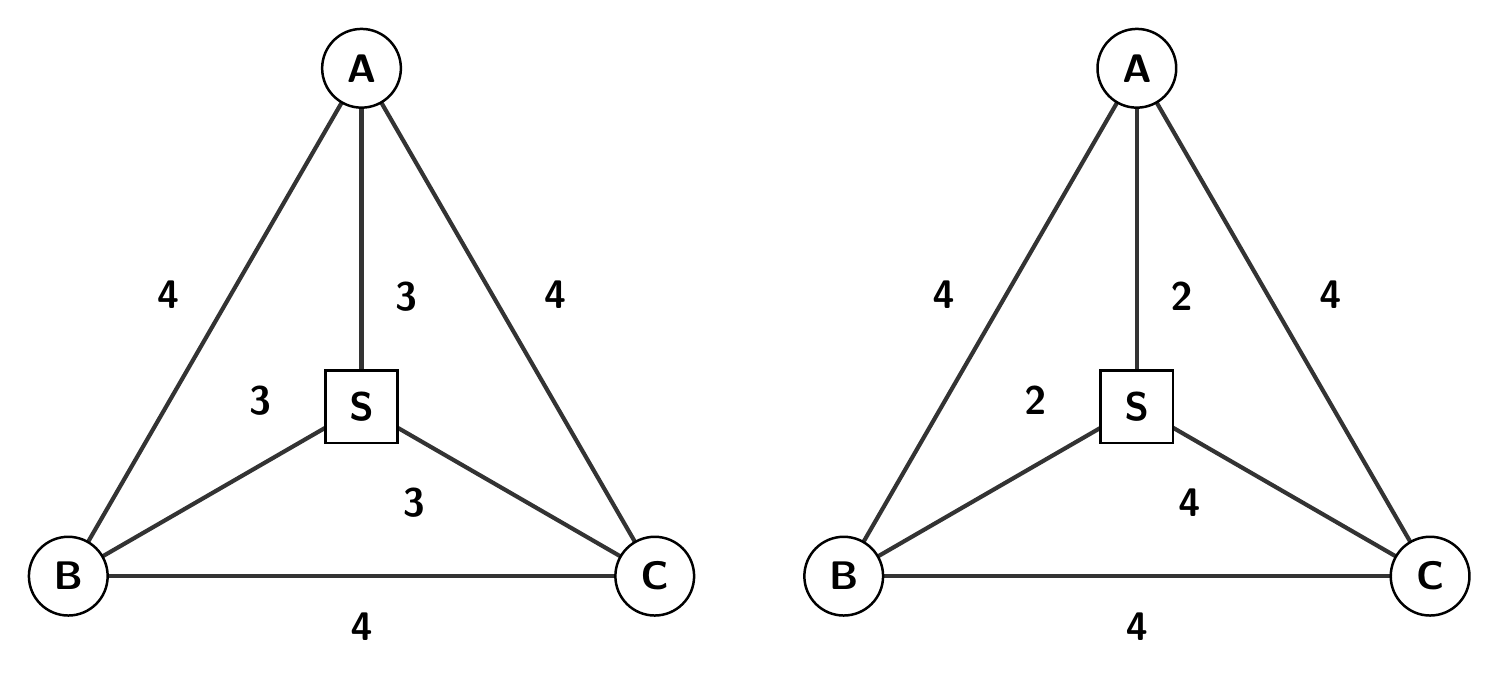
\begin{tikzpicture}[x=1mm,y=1mm]
\draw[line width=1.5pt, black!80] (42.24,73.96) -- (5.00,9.46);
\draw[line width=1.5pt, black!80] (5.00,9.46) -- (79.48,9.46);
\draw[line width=1.5pt, black!80] (42.24,73.96) -- (79.48,9.46);
\draw[line width=1.5pt, black!80] (42.24,30.96) -- (42.24,73.96);
\draw[line width=1.5pt, black!80] (42.24,30.96) -- (5.00,9.46);
\draw[line width=1.5pt, black!80] (42.24,30.96) -- (79.48,9.46);
\node[fill=white, inner sep=0, minimum width=4.40mm, minimum height=6.00mm, font=\Large\bfseries] at (17.67,45.15) {4};
\node[fill=white, inner sep=0, minimum width=4.40mm, minimum height=6.00mm, font=\Large\bfseries] at (42.24,3.00) {4};
\node[fill=white, inner sep=0, minimum width=4.40mm, minimum height=6.00mm, font=\Large\bfseries] at (66.81,45.15) {4};
\node[fill=white, inner sep=0, minimum width=4.40mm, minimum height=6.00mm, font=\Large\bfseries] at (47.90,44.94) {3};
\node[fill=white, inner sep=0, minimum width=4.40mm, minimum height=6.00mm, font=\Large\bfseries] at (29.35,31.79) {3};
\node[fill=white, inner sep=0, minimum width=4.40mm, minimum height=6.00mm, font=\Large\bfseries] at (48.90,18.85) {3};
\node[circle, draw, line width=0.9pt, fill=white, minimum size=10.00mm, inner sep=0, font=\Large\bfseries] at (42.24,73.96) {A};
\node[circle, draw, line width=0.9pt, fill=white, minimum size=10.00mm, inner sep=0, font=\Large\bfseries] at (5.00,9.46) {B};
\node[circle, draw, line width=0.9pt, fill=white, minimum size=10.00mm, inner sep=0, font=\Large\bfseries] at (79.48,9.46) {C};
\node[rectangle, draw, line width=0.9pt, fill=white, minimum size=9.20mm, inner sep=0, font=\Large\bfseries] at (42.24,30.96) {S};
\draw[line width=1.5pt, black!80] (140.71,73.96) -- (103.48,9.46);
\draw[line width=1.5pt, black!80] (103.48,9.46) -- (177.95,9.46);
\draw[line width=1.5pt, black!80] (140.71,73.96) -- (177.95,9.46);
\draw[line width=1.5pt, black!80] (140.71,30.96) -- (140.71,73.96);
\draw[line width=1.5pt, black!80] (140.71,30.96) -- (103.48,9.46);
\draw[line width=1.5pt, black!80] (140.71,30.96) -- (177.95,9.46);
\node[fill=white, inner sep=0, minimum width=4.40mm, minimum height=6.00mm, font=\Large\bfseries] at (116.15,45.15) {4};
\node[fill=white, inner sep=0, minimum width=4.40mm, minimum height=6.00mm, font=\Large\bfseries] at (140.71,3.00) {4};
\node[fill=white, inner sep=0, minimum width=4.40mm, minimum height=6.00mm, font=\Large\bfseries] at (165.28,45.15) {4};
\node[fill=white, inner sep=0, minimum width=4.40mm, minimum height=6.00mm, font=\Large\bfseries] at (146.38,44.94) {2};
\node[fill=white, inner sep=0, minimum width=4.40mm, minimum height=6.00mm, font=\Large\bfseries] at (127.82,31.79) {2};
\node[fill=white, inner sep=0, minimum width=4.40mm, minimum height=6.00mm, font=\Large\bfseries] at (147.37,18.85) {4};
\node[circle, draw, line width=0.9pt, fill=white, minimum size=10.00mm, inner sep=0, font=\Large\bfseries] at (140.71,73.96) {A};
\node[circle, draw, line width=0.9pt, fill=white, minimum size=10.00mm, inner sep=0, font=\Large\bfseries] at (103.48,9.46) {B};
\node[circle, draw, line width=0.9pt, fill=white, minimum size=10.00mm, inner sep=0, font=\Large\bfseries] at (177.95,9.46) {C};
\node[rectangle, draw, line width=0.9pt, fill=white, minimum size=9.20mm, inner sep=0, font=\Large\bfseries] at (140.71,30.96) {S};
\end{tikzpicture}
\end{center}\par

\vspace{16mm}
\par\begin{center}
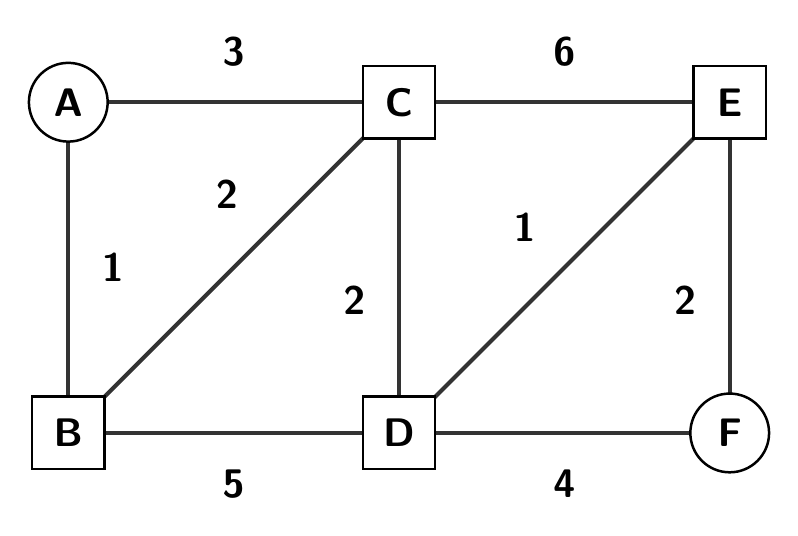
\begin{tikzpicture}[x=1mm,y=1mm]
\draw[line width=1.5pt, black!80] (5.00,51.46) -- (5.00,9.46);
\draw[line width=1.5pt, black!80] (5.00,9.46) -- (47.00,51.46);
\draw[line width=1.5pt, black!80] (5.00,51.46) -- (47.00,51.46);
\draw[line width=1.5pt, black!80] (47.00,51.46) -- (47.00,9.46);
\draw[line width=1.5pt, black!80] (47.00,9.46) -- (89.00,51.46);
\draw[line width=1.5pt, black!80] (89.00,51.46) -- (89.00,9.46);
\draw[line width=1.5pt, black!80] (47.00,9.46) -- (89.00,9.46);
\draw[line width=1.5pt, black!80] (5.00,9.46) -- (47.00,9.46);
\draw[line width=1.5pt, black!80] (47.00,51.46) -- (89.00,51.46);
\node[fill=white, inner sep=0, minimum width=4.40mm, minimum height=6.00mm, font=\Large\bfseries] at (10.66,30.46) {1};
\node[fill=white, inner sep=0, minimum width=4.40mm, minimum height=6.00mm, font=\Large\bfseries] at (25.15,39.71) {2};
\node[fill=white, inner sep=0, minimum width=4.40mm, minimum height=6.00mm, font=\Large\bfseries] at (26.00,57.93) {3};
\node[fill=white, inner sep=0, minimum width=4.40mm, minimum height=6.00mm, font=\Large\bfseries] at (41.34,26.26) {2};
\node[fill=white, inner sep=0, minimum width=4.40mm, minimum height=6.00mm, font=\Large\bfseries] at (62.95,35.51) {1};
\node[fill=white, inner sep=0, minimum width=4.40mm, minimum height=6.00mm, font=\Large\bfseries] at (83.34,26.26) {2};
\node[fill=white, inner sep=0, minimum width=4.40mm, minimum height=6.00mm, font=\Large\bfseries] at (68.00,3.00) {4};
\node[fill=white, inner sep=0, minimum width=4.40mm, minimum height=6.00mm, font=\Large\bfseries] at (26.00,3.00) {5};
\node[fill=white, inner sep=0, minimum width=4.40mm, minimum height=6.00mm, font=\Large\bfseries] at (68.00,57.93) {6};
\node[circle, draw, line width=0.9pt, fill=white, minimum size=10.00mm, inner sep=0, font=\Large\bfseries] at (5.00,51.46) {A};
\node[rectangle, draw, line width=0.9pt, fill=white, minimum size=9.20mm, inner sep=0, font=\Large\bfseries] at (47.00,51.46) {C};
\node[rectangle, draw, line width=0.9pt, fill=white, minimum size=9.20mm, inner sep=0, font=\Large\bfseries] at (89.00,51.46) {E};
\node[rectangle, draw, line width=0.9pt, fill=white, minimum size=9.20mm, inner sep=0, font=\Large\bfseries] at (5.00,9.46) {B};
\node[rectangle, draw, line width=0.9pt, fill=white, minimum size=9.20mm, inner sep=0, font=\Large\bfseries] at (47.00,9.46) {D};
\node[circle, draw, line width=0.9pt, fill=white, minimum size=10.00mm, inner sep=0, font=\Large\bfseries] at (89.00,9.46) {F};
\end{tikzpicture}
\end{center}\par

\newpage

\prob{10} Find a cheapest network on this map. Then start again with AB and BC bought. A change is buying one link, returning one link, or swapping one bought link for one that is not bought, as long as A, B and C stay joined. Can you get from AB and BC to a cheapest network by changes that never make the total cost more than 8? Explain.

\par\begin{center}
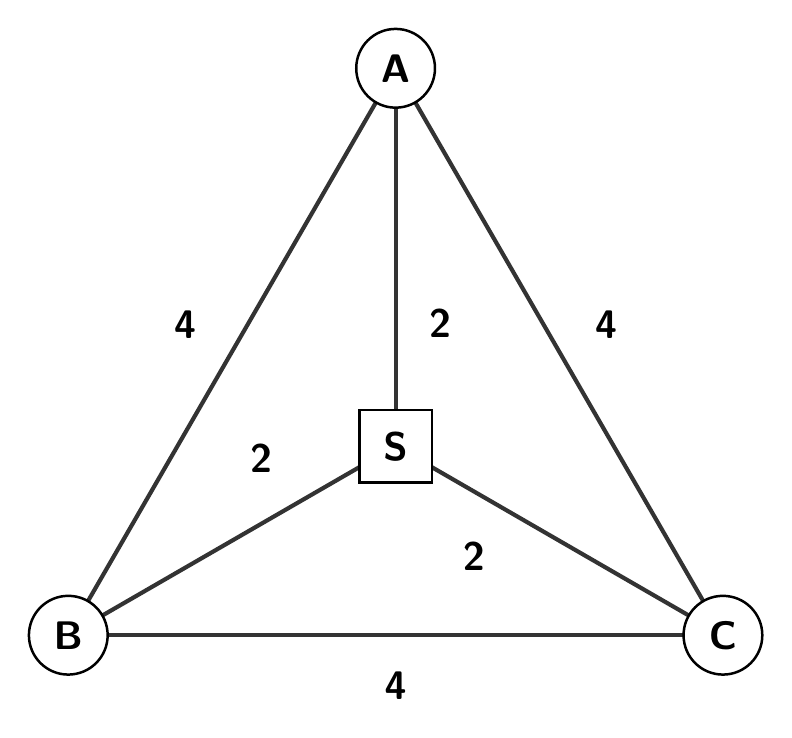
\begin{tikzpicture}[x=1mm,y=1mm]
\draw[line width=1.5pt, black!80] (46.57,81.46) -- (5.00,9.46);
\draw[line width=1.5pt, black!80] (5.00,9.46) -- (88.14,9.46);
\draw[line width=1.5pt, black!80] (46.57,81.46) -- (88.14,9.46);
\draw[line width=1.5pt, black!80] (46.57,33.46) -- (46.57,81.46);
\draw[line width=1.5pt, black!80] (46.57,33.46) -- (5.00,9.46);
\draw[line width=1.5pt, black!80] (46.57,33.46) -- (88.14,9.46);
\node[fill=white, inner sep=0, minimum width=4.40mm, minimum height=6.00mm, font=\Large\bfseries] at (19.83,48.90) {4};
\node[fill=white, inner sep=0, minimum width=4.40mm, minimum height=6.00mm, font=\Large\bfseries] at (46.57,3.00) {4};
\node[fill=white, inner sep=0, minimum width=4.40mm, minimum height=6.00mm, font=\Large\bfseries] at (73.30,48.90) {4};
\node[fill=white, inner sep=0, minimum width=4.40mm, minimum height=6.00mm, font=\Large\bfseries] at (52.23,49.06) {2};
\node[fill=white, inner sep=0, minimum width=4.40mm, minimum height=6.00mm, font=\Large\bfseries] at (29.48,31.87) {2};
\node[fill=white, inner sep=0, minimum width=4.40mm, minimum height=6.00mm, font=\Large\bfseries] at (56.50,19.46) {2};
\node[circle, draw, line width=0.9pt, fill=white, minimum size=10.00mm, inner sep=0, font=\Large\bfseries] at (46.57,81.46) {A};
\node[circle, draw, line width=0.9pt, fill=white, minimum size=10.00mm, inner sep=0, font=\Large\bfseries] at (5.00,9.46) {B};
\node[circle, draw, line width=0.9pt, fill=white, minimum size=10.00mm, inner sep=0, font=\Large\bfseries] at (88.14,9.46) {C};
\node[rectangle, draw, line width=0.9pt, fill=white, minimum size=9.20mm, inner sep=0, font=\Large\bfseries] at (46.57,33.46) {S};
\end{tikzpicture}
\end{center}\par

\newpage

\prob{11} Find a cheapest network on this map. In a cheapest network on any map, can a square place have just one bought link? If four places are circled, what is the largest number of square places that can have three or more bought links in a cheapest network? Explain.

\par\begin{center}
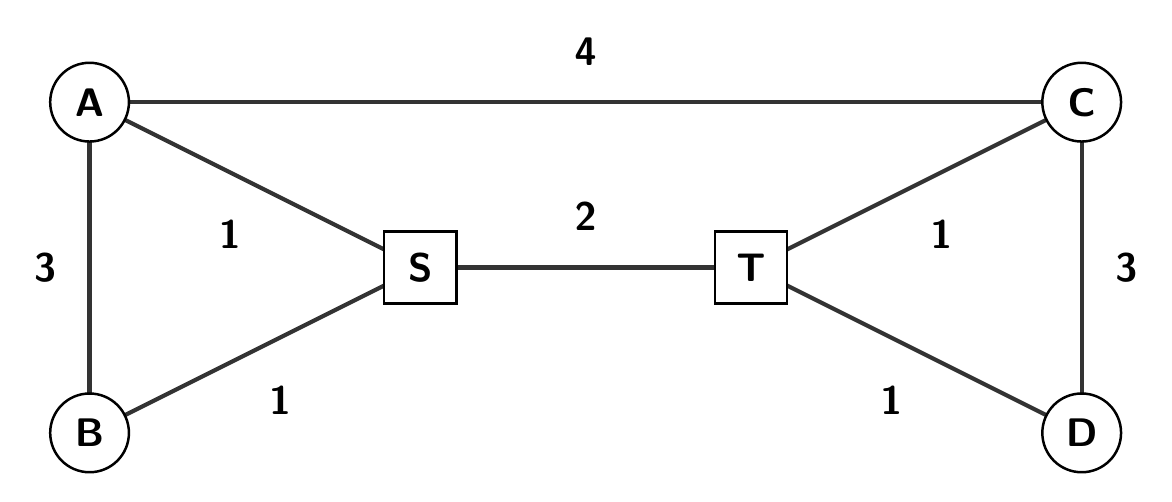
\begin{tikzpicture}[x=1mm,y=1mm]
\draw[line width=1.5pt, black!80] (7.86,47.00) -- (49.86,26.00);
\draw[line width=1.5pt, black!80] (7.86,5.00) -- (49.86,26.00);
\draw[line width=1.5pt, black!80] (49.86,26.00) -- (91.86,26.00);
\draw[line width=1.5pt, black!80] (91.86,26.00) -- (133.86,47.00);
\draw[line width=1.5pt, black!80] (91.86,26.00) -- (133.86,5.00);
\draw[line width=1.5pt, black!80] (7.86,47.00) -- (7.86,5.00);
\draw[line width=1.5pt, black!80] (133.86,47.00) -- (133.86,5.00);
\draw[line width=1.5pt, black!80] (7.86,47.00) -- (133.86,47.00);
\node[fill=white, inner sep=0, minimum width=4.40mm, minimum height=6.00mm, font=\Large\bfseries] at (25.68,30.12) {1};
\node[fill=white, inner sep=0, minimum width=4.40mm, minimum height=6.00mm, font=\Large\bfseries] at (32.05,9.12) {1};
\node[fill=white, inner sep=0, minimum width=4.40mm, minimum height=6.00mm, font=\Large\bfseries] at (70.86,32.46) {2};
\node[fill=white, inner sep=0, minimum width=4.40mm, minimum height=6.00mm, font=\Large\bfseries] at (116.05,30.12) {1};
\node[fill=white, inner sep=0, minimum width=4.40mm, minimum height=6.00mm, font=\Large\bfseries] at (109.68,9.12) {1};
\node[fill=white, inner sep=0, minimum width=4.40mm, minimum height=6.00mm, font=\Large\bfseries] at (2.20,26.00) {3};
\node[fill=white, inner sep=0, minimum width=4.40mm, minimum height=6.00mm, font=\Large\bfseries] at (139.53,26.00) {3};
\node[fill=white, inner sep=0, minimum width=4.40mm, minimum height=6.00mm, font=\Large\bfseries] at (70.86,53.46) {4};
\node[circle, draw, line width=0.9pt, fill=white, minimum size=10.00mm, inner sep=0, font=\Large\bfseries] at (7.86,47.00) {A};
\node[circle, draw, line width=0.9pt, fill=white, minimum size=10.00mm, inner sep=0, font=\Large\bfseries] at (7.86,5.00) {B};
\node[rectangle, draw, line width=0.9pt, fill=white, minimum size=9.20mm, inner sep=0, font=\Large\bfseries] at (49.86,26.00) {S};
\node[rectangle, draw, line width=0.9pt, fill=white, minimum size=9.20mm, inner sep=0, font=\Large\bfseries] at (91.86,26.00) {T};
\node[circle, draw, line width=0.9pt, fill=white, minimum size=10.00mm, inner sep=0, font=\Large\bfseries] at (133.86,47.00) {C};
\node[circle, draw, line width=0.9pt, fill=white, minimum size=10.00mm, inner sep=0, font=\Large\bfseries] at (133.86,5.00) {D};
\end{tikzpicture}
\end{center}\par

\vspace{50mm}
\prob{12} Lee says that on a map with no squares, a network with no loop must be a cheapest network if, for every two places, no route on the map between them has a cheaper most expensive link than the route along the network. Is Lee right? Explain.

\end{document}
